\documentclass{article}

\usepackage[utf8]{inputenc}
\usepackage{amsmath, amssymb, amsthm}
\usepackage[dvipsnames]{xcolor}
\usepackage{color}
\usepackage{tikz}
\usepackage{array}
\usepackage{pgfmath}
\usepackage{soul}
\usepackage{multirow}
\usepackage{colortbl}
\usepackage{pgfplots}
\usepackage{ulem}
\usepackage{extpfeil}
\usepackage[hidelinks]{hyperref}

\pgfplotsset{compat=1.18}
\usetikzlibrary{matrix}


\definecolor{dgr}{rgb}{0.72, 0.53, 0.04}
\definecolor{maroon}{rgb}{0.5, 0.0, 0.0}


\newcommand{\smsk}{\vspace{3px}}
\newcommand{\mesk}{\vspace{10px}}

\newcommand{\smsp}{\phantom{\hspace{3px}}}
\newcommand{\mesp}{\phantom{\hspace{10px}}}

\newcommand{\red}[1]{\textcolor{red}{#1}}
\newcommand{\gray}[1]{\textcolor{gray}{#1}}
\newcommand{\blue}[1]{\textcolor{blue}{#1}}
\newcommand{\green}[1]{\textcolor{green}{#1}}
\newcommand{\dgr}[1]{\textcolor{dgr}{#1}}
\newcommand{\maroon}[1]{\textcolor{maroon}{#1}}
\newcommand{\cyan}[1]{\textcolor{cyan}{#1}}

\newcommand{\hcyan}[1]{\colorbox{cyan}{#1}}
\newcommand{\hgreen}[1]{\colorbox{green}{#1}}

\newcommand{\ex}{\green{\textbf{Beispiel: }}}
\newcommand{\de}[1]{\red{\textbf{Definition: }}\begin{quote}#1\end{quote}}
\newcommand{\an}[1]{\blue{\textbf{Bemerkung: }}\begin{quote}#1\end{quote}}
\newcommand{\prop}[1]{\dgr{\textbf{Proposition: }}\begin{quote}#1\end{quote}}
\newcommand{\se}[1]{\dgr{\textbf{Satz: }}\begin{quote}#1\end{quote}}
\newcommand{\lem}[1]{\dgr{\textbf{Lemma: }}\begin{quote}#1\end{quote}}
\newcommand{\cl}[1]{\dgr{\textbf{Behauptung: }}\begin{quote}#1\end{quote}}
\newcommand{\co}[1]{\dgr{\textbf{Korollar: }}\begin{quote}#1\end{quote}}
\newcommand{\pr}[1]{\maroon{\textbf{Beweis: }}\begin{quote}#1\end{quote}\qed}

\newcommand{\n}[1]{\overline{#1}}
\newcommand{\N}{\mathbb{N}}
\newcommand{\Z}{\mathbb{Z}}
\newcommand{\Q}{\mathbb{Q}}
\newcommand{\R}{\mathbb{R}}
\newcommand{\C}{\mathbb{C}}
\newcommand{\vst}{\smsp \vline \smsp}
\renewcommand{\st}{\smsp | \smsp}

\newcommand{\xor}{\mathbin{\vartriangle}}
\newcommand{\vvec}[2]{\begin{pmatrix}#1\\#2\end{pmatrix}}
\newcommand{\vvvec}[3]{\begin{pmatrix}#1\\#2\\#3\end{pmatrix}}

\renewcommand{\mod}{\text{ mod }}
\newcommand{\spann}[1]{\left\langle#1\right\rangle}
\newcommand{\col}{\text{col}}
\newcommand{\row}{\text{row}}
\newcommand{\rg}{\text{rg}}
\newcommand{\im}{\text{Im}}
\newcommand{\ggt}{\text{ggT}}

\newcommand{\bs}{\backslash}


\setlength{\parindent}{0pt}
\setlength{\parskip}{3pt}


\title{Diskrete Strukturen}
\author{Daniel}
\date{October 2024}

\begin{document}

\maketitle
\tableofcontents

\newpage
\section{Mengen}

\de{Eine \red{Menge} ist eine Zusammenfassung von bestimmten, wohlunterschiedenen Objekten unserer Anschauung oder unseres Denkens zu einem Ganzen, die dann die Elemente der Menge genannt werden.}

\begin{table}[ht]
    \centering
    \begin{tabular}{c p{9cm}}
        \textbf{\red{Symbolik}} & \textbf{\red{Bedeutung}}\\
        $e \in M$ & Das Element $e$ ist Element der Menge $M$\\
        $e \notin M $ & Das Element $e$ ist kein Element der Menge $M$\\\
        $\emptyset$ oder $\{\}$ & Leere Menge\\
        $A \subseteq B$ & $A$ ist $Teilmenge$ von $B$, d.h. jedes Element von $A$ ist auch Element von $B$\\
        $A \subset B$ & $A$ ist $echte$ $Teilmenge$ von $B$, d.h. jedes Element von $A$ ist auch Element von $B$, aber $A \neq B$ ($A \subset B \implies A \subseteq B$)
    \end{tabular}
\end{table}

\ex Es ist eine Menge $M = \{1, 2, 3\}$ gegeben. Dann gilt:
\begin{itemize}
    \item $M = \{3, 1, 2\} = \{1, 1, 2, 3, 3, 3, 3\}$
    \item $1 \in M$ und $4 \notin M$
    \item $\emptyset \subset M$
    \item $\{1\} \notin M$, aber $\{1\} \subset M$
\end{itemize}

\an{Keine Menge kann Element von sich selbst sein! $ \rightarrow M \notin M$}

\phantomsection
\addcontentsline{toc}{subsection}{\hspace{11cm}}
\subsubsection{Quantoren}
\an{Um (Teil-)Mengen zu beschreiben oder Aussagen zu formulieren, werden oft Quantoren benutzt}

\begin{table}[ht]
    \centering
    \begin{tabular}{c p{7cm}}
        \textbf{\red{Quantor}} & \textbf{\red{Bedeutung}}\\
        $Allquantor$ $\forall$ & "für alle" bzw. "für jedes"\\
        $Existenzquantor$ $\exists$ & "es gibt (mindestens) ein" bzw. "es existiert (mindestens) ein"\\
        $Eindeutigkeitsquantor$ $\exists!$ & "es gibt genau ein" bzw. "es existiert genau ein"\\
        $\nexists$ & "es gibt kein" bzw. "es existiert kein" (Negation des Existenzquantors)
    \end{tabular}
\end{table}

\an{Mengenbeziehungen können auch durch Quantoren dargestellt werden:}

\begin{equation*}
    \begin{array}{lcl}
        A \subseteq B & \iff & \forall e \in A \vst e \in B\\
                      & \iff & \nexists e \in A\vst e \notin B\\
                      & \iff & \forall e_1 \in A \: \exists e_2 \in B \vst e_1 = e_2\\
        A = b         & \iff & (A \subseteq B) \: \land \: (B \subseteq A)\\
                      & \iff & (\forall e \in A \vst e \in B) \land (\forall e \in B \vst e \in A)
    \end{array}
\end{equation*}

\ex Im Folgenden sind einige Mengen aufgelistet

\begin{itemize}
    \item natürliche Zahlen $\N = \{0, 1, 2, 3, 4, 5, \dots\}$\\
    $\forall x \in \N \: \exists!y \in \N \vst y = x + 1$\\
    $\exists! x \in \N \vst x - 1 \notin \N$\\
    Sei $A \subseteq \N$ mit $0 \in A$ und $\forall x \in A \vst x + 1 \in A$. Dann gilt $A = \N$ (Péano-Axiome, axiomatische Definition der natürlichen Zahlen)
    \item ganze Zahlen $\Z = \{\dots, -2, -1, 0, 1, 2, \dots\}$
    \item rationale Zahlen $\Q = \{\frac{a}{b} \vst a \in \Z, b \in \Z, b \neq 0\}$
\end{itemize}

Mengen können auch andere Mengen als Elemente enthalten:\\
\ex $N = \{0, \{1, 2\}\}$

\begin{itemize}
    \item $\{1, 2\} \in N$
    \item $\{\{1, 2\}\} \subset N$
    \item $\{1\} \notin N$
    \item $\{1, 2\} \nsubseteq N$
\end{itemize}

\subsubsection{Die Kardinalität einer Menge}

\de{Die \red{Kardinalität} $|M|$, auch Mächtigkeit, einer Menge M beschreibt die Anzahl der Elemente in M.}

\ex
\begin{itemize}
    \item $|\{0, 1, 2\}| = |\{0, 0, 0, 1, 2, 2\}| = 3$
    \item $|\{0, \{1, 2\}\}| = 2$
    \item $|\emptyset| = |\{\}| = 0$
    \item $|\{\emptyset\}| = |\{\{\}\}| = 1$
    \item $|\N| = |\Q| = \infty$
\end{itemize}

\subsection{Mengen durch Aussonderung}

\an{Mengen können geschrieben werden, indem Bedingungen an ihre Elemente geknüpft werden}

\ex
\begin{itemize}
    \item \{$x \vst x$ erfüllt die Bedingung *\}
    \item \{$x \in M \vst x$ erfüllt die Bedingung *\}
    \item $\Q = \{\frac{a}{b} \vst a \in \Z, b \in \Z, b \neq 0\}$
    \item \{$x \in \N \vst x \leq 2\} = \{0, 1, 2$\}
    \item \{$x \in \Z \vst \exists y \in \Z \vst x = 3y\} = \{\dots, -9, -6, -3, 0, 3, 6, 9, \dots\}$
\end{itemize}

\subsection{Mengenoperationen}

\begin{table}[h]
    \centering
    \begin{tabular}{m{7.5cm} m{3.7cm}}
        \centering\textbf{\red{Schreibweise}} & \textbf{\red{Mengen-Diagramm}}\\
        \centering
        $B \subset A$&
        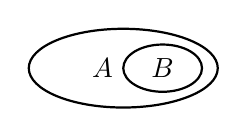
\begin{tikzpicture}
            \draw[thick, black] (0, 0) ellipse (1.2 and 0.5) node[left] {$A$};
            \draw[thick, black] (0.5, 0) ellipse (0.5 and 0.3) node {$B$};
        \end{tikzpicture}\\
        \(
            \begin{array}{lcl}
                 Schnitt: A \cap B  & = & \{ x \vst x \in A \land x \in B \} \\
                                    & = & \{ x \in A  \vst x \in B \}\\
                                    & = & \{x \in B \vst x \in A\}
            \end{array}
        \) &
        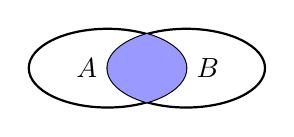
\begin{tikzpicture}
            \draw[thick, black] (0, 0) ellipse (1 and 0.5) node[left] {$A$};
            \draw[thick, black] (1, 0) ellipse (1 and 0.5) node[right] {$B$};
            \begin{scope}
                \clip (0, 0) ellipse (1 and 0.5);
                \fill[blue!40] (1, 0) ellipse (1 and 0.5);
            \end{scope}
        \end{tikzpicture}\\
        \centering
        $Vereinigung: A \cup B = \{x \vst x \in A \lor x \in B\}$ &
        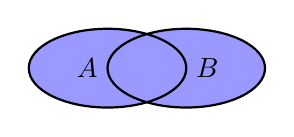
\begin{tikzpicture}
            \fill[fill=blue!40] (0, 0) ellipse (1 and 0.5) node[left] {$A$};
            \fill[fill=blue!40] (1, 0) ellipse (1 and 0.5) node[right] {$B$};
            \draw[thick, black] (0, 0) ellipse (1 and 0.5);
            \draw[thick, black] (1, 0) ellipse (1 and 0.5);
        \end{tikzpicture}\\
        \centering
        $Differenz: A \bs B = \{x \in A \vst x \notin B\}$ &
        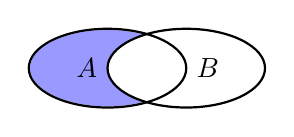
\begin{tikzpicture}
            \fill[thick, fill=blue!40, draw=white] (0, 0) ellipse (1 and 0.5) node[left] {$A$};
            \filldraw[thick, draw=black, fill=white] (1, 0) ellipse (1 and 0.5) node[right] {$B$};
            \draw[thick, black] (0, 0) ellipse (1 and 0.5);
        \end{tikzpicture}\\
        \centering
        $symmetrische$ $Differenz:$ $A \Delta B = \{x \in A \cup B \vst x \notin A  \cap B\}$ &
        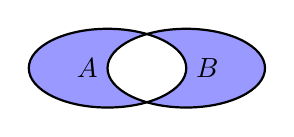
\begin{tikzpicture}
            \fill[draw=white, fill=blue!40] (0, 0) ellipse (1 and 0.5) node[left] {$A$};
            \fill[draw=white, fill=blue!40] (1, 0) ellipse (1 and 0.5) node[right] {$B$};
            \begin{scope}
                \clip (0, 0) ellipse (1 and 0.5);
                \fill[white] (1, 0) ellipse (1 and 0.5);
            \end{scope}
            \draw[thick, black] (0, 0) ellipse (1 and 0.5);
            \draw[thick, black] (1, 0) ellipse (1 and 0.5);
        \end{tikzpicture}\\
        \centering
        \(
            \begin{array}{lcl}
                 Disjunktion: A \perp B  & \iff & A \cap B = \emptyset \\
                                         & \iff & \forall x \in A \vst x \notin B\\
            \end{array}
        \) &
        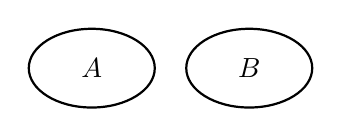
\begin{tikzpicture}
            \draw[thick, black] (0, 0) ellipse (0.8 and 0.5) node {$A$};
            \draw[thick, black] (2, 0) ellipse (0.8 and 0.5) node {$B$};
        \end{tikzpicture}\\
    \end{tabular}
\end{table}

\newpage
\subsection{Rechenregeln}

\begin{itemize}
    \item Schnitt und Vereinigung von Mengen sind \textcolor{red}{idempotent}:
    \begin{equation*}
        \begin{array}{lcl}
            A \cap A & = & A\\
            A \cup A & = & A
        \end{array}
    \end{equation*}
    \item Schnitt und Vereinigung von Mengen sind \textcolor{red}{kommutativ}:
    \begin{equation*}
        \begin{array}{lcl}
            A \cap B & = & B \cap A\\
            A \cup B & = & B \cup A
        \end{array}
    \end{equation*}
    \item Schnitt und Vereinigung von Mengen sind \textcolor{red}{assoziativ}:
    \begin{equation*}
        \begin{array}{lcl}
            A \cap (B \cap C) & = & (A \cap B) \cap C\\
            A \cup (B \cup C) & = & (A \cup B) \cup C
        \end{array}
    \end{equation*}
    \item Schnitt ist \textcolor{red}{distributiv} über Vereinigung:
    \begin{equation*}
        A \cap (B \cup C) = (A \cap B) \cup (A \cap C)
    \end{equation*}
    \item Vereinigung ist \textcolor{red}{distributiv} über Schnitt:
    \begin{equation*}
        A \cup (B \cap C) = (A \cup B) \cap (A \cup C)
    \end{equation*}
\end{itemize}

\an{Vereinigung und Schnitt können auch über beliebig viele Mengen gebildet werden:}

\begin{itemize}
    \item Sei I eine Menge ("Indexmenge", die alle Mengen markiert, die vereinigt werden) und für jedes $i \in I$ sei $M_i$ eine Menge, so gilt für die \textcolor{red}{Vereinigung} dieser Mengen:
    \begin{equation*}
        \bigcup_{i \in I} M_i := \{x \vst \exists i \in I \vst x \in M_i\}
    \end{equation*}
    \textbf{Bedeutung:} Die Vereinigung der Mengen $M_i$ ist die Menge aller Elemente x, die in mindestens einer der Mengen $M_i$ enthalten sind.
    \item Sei I eine Menge und für jedes $i \in I$ sei $M_i$ eine Menge, so gilt für den \textcolor{red}{Schnitt} dieser Mengen:
    \begin{equation*}
        \bigcap_{i \in I} M_i := \{x \vst \forall i \in I \vst x \in M_i\}
    \end{equation*}
    \textbf{Bedeutung:} Der Schnitt der Mengen $M_i$ ist die Menge aller Elemente x, die in allen Mengen $M_i$ enthalten sind.
\end{itemize}

\subsection*{Exkursion: Definieren}

\de{Das Symbol \red{$:=$} bedeutet so viel wie "wird an dieser Stelle definiert als". Dabei wird einem Objekt, welches noch keine Bedeutung hat, auf der linken Seite des Operators die Bedeutung eines Ausdrucks auf der rechten Seite des Operators zugewiesen}

Nehme an, dass $|K| < \infty$, d.h. die Menge $I = \{i_1, i_2, i_3, \dots, i_n\}$ hat endlich viele Elemente
\begin{itemize}
    \item Die Summe ist dann definiert als
    \begin{equation*}
        \sum_{i \in I} x_i := x_{i_1} + x_{i_2} + x_{i_3} + \dots + x_{i_n} \quad mit \sum_{i \in \emptyset} x_i := 0
    \end{equation*}
    \item Das Produkt ist dann definiert als
    \begin{equation*}
        \prod_{i \in I} x_i := x_{i_1} \cdot x_{i_2} \cdot x_{i_3} \cdot \dots \cdot x_{i_n} \quad mit \prod_{i \in \emptyset} x_i := 1
    \end{equation*}
    \item Praktisch wird dabei meistens $I = \{0, 1 , 2, \dots, n\}$ verwendet, sodass gilt
    \begin{equation*}
        \begin{split}
            \sum_{i = 0}^n x_i & := x_0 + x_1 + x_2 + \dots + x_n\\
            \prod_{i = 0}^n x_i & := x_0 \cdot x_1 \cdot x_2 \cdot \dots \cdot x_n
        \end{split}
    \end{equation*}
\end{itemize}

\ex
\begin{equation*}
    \begin{split}
        \sum_{i = 0}^3 i^2 & = 0^2 + 1^2 + 2^2 + 3^2 = 0 + 1 + 4 + 9 = 14\\
        \prod_{i = 0}^3 i^2 & = 0^2 \cdot 1^2 \cdot 2^2 \cdot 3^2 = 0 \cdot 1 \cdot 4 \cdot 9 = 0
    \end{split}
\end{equation*}

\subsection{Mengenkomplement}

\de{Sei $U$ eine Menge ("Universum") und $A, B \subseteq U$, so schreiben wir das \red{Komplement}, auch Mengenkomplement, von $A$ als $\n{A} := U \bs A$.}

\newpage
\subsubsection{De-Morgansche Regeln}
\an{Für Komplementärmengen gelten die De-Morgan'schen Regeln:}

\begin{table}[h]
    \centering
    \begin{tabular}{m{4cm} m{5cm}}
        $\n{A \cup B} = \n{A} \cap \n{B}$ &
        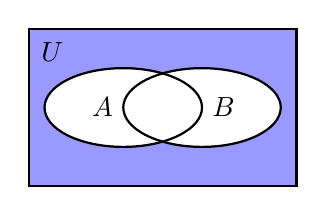
\begin{tikzpicture}
            \filldraw[thick, fill = blue!40, draw = black] (0, 0) rectangle (3.4cm, 2cm);
            \fill[white] (1.2, 1) ellipse (1 and 0.5);
            \filldraw[thick, draw=black, fill=white] (2.2, 1) ellipse (1 and 0.5) node[right] {$B$};
            \draw[thick, black] (1.2, 1) ellipse (1 and 0.5) node[left] {$A$};
            \node at (0.3, 1.7) {$U$};
        \end{tikzpicture}\\
        $\n{A \cap B} = \n{A} \cup \n{B}$ &
        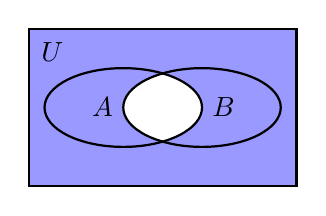
\begin{tikzpicture}
            \filldraw[thick, fill = blue!40, draw = black] (0, 0) rectangle (3.4cm, 2cm);
            \node at (0.3, 1.7) {$U$};
            \begin{scope}
                \clip (1.2, 1) ellipse (1 and 0.5);
                \fill[white] (2.2, 1) ellipse (1 and 0.5);
            \end{scope}
            \draw[thick, black] (1.2, 1) ellipse (1 and 0.5) node[left] {$A$};
            \draw[thick, draw=black] (2.2, 1) ellipse (1 and 0.5) node[right] {$B$};
        \end{tikzpicture}\\
    \end{tabular}
\end{table}

\subsection{Paare und Produkte}

\de{Ein \red{geordnetes Paar $(a, b)$} ist eine Zusammenfassung von zwei Objekten $a$ und $b$ zu einem Ganzen, wobei die Reihenfolge der Objekte eine Rolle spielt:}

\begin{center}
    Seien $A, B$ Mengen. Sei $a \in A$ und $b \in B$. So schreiben wir:
    \begin{equation*}
        (a, b) := \{\{a\}, \{a, b\}\}
    \end{equation*}
    Dabei stellt $a$ in der Menge das erste Objekt des Paares dar.
\end{center}

\subsubsection{Kartesisches Produkt}
\de{Das \red{Kartesische Produkt $A \times B$} zweier Mengen $A$ und $B$ ist die Menge aller geordneten Paare $(a, b)$ aus Elementen der Mengen, wobei $a \in A$ und $b \in B$:}
\begin{equation*}
    A \times B := \{(a, b) \vst a \in A, b \in B\}
\end{equation*}

\ex Seien $A = \{1, 2\}$ und $B = \{3, 4\}$. Dann gilt:
\begin{equation*}
    A \times B = \{(1, 3), (1, 4), (2, 3), (2, 4)\}
\end{equation*}

\newpage
\an{Wenn A und B endlich sind, also $|A| < \infty$ und $|B| < \infty$, so gilt:}
\begin{equation*}
    |A \times B| = |A| \cdot |B|
\end{equation*}

\ex Auf $\Z$ (im Bereich der ganzen Zahlen) ist $\leq$ folgendermaßen definiert:
\begin{equation*}
    \begin{array}{lcl}
        x \leq y & := & \{(x, y) \in \Z \times \Z \vst y - x \in \N\}\\
                 & := & \{(x, y) \in \Z^2 \vst \exists! z \in \N: x + z = y\}
    \end{array}
\end{equation*}
Es existiert (nach der zweiten Definition) also genau eine Zahl $z$ in $\N$, sodass $x + z = y$.

\subsubsection{Potenzmengen}

\de{Die \red{Potenzmenge P(M)} einer Menge $M$ ist die Menge aller Teilmengen der Menge $M$}

\ex Sei $M$ die Menge $\{0, 1, 2\}$, so gilt für die Potenzmenge $P(M)$ der Menge M:
\begin{equation*}
    P(M) = \{\emptyset, \{0\}, \{1\}, \{2\}, \{0, 1\}, \{0, 2\}, \{1, 2\}, \{0, 1, 2\}\}
\end{equation*}

\an{Für eine Menge $M$ mit $|M| < \infty$ gilt:}
\begin{equation*}
    |P(M)| = 2^{|M|}
\end{equation*}
\begin{quote}
    Um eine Teilmenge $M_{Teil} \subseteq M$ auszuwählen gibt es für jedes Element $e \in M$ die zwei Möglichkeiten $e \in M_{Teil}$ und $e \notin M_{Teil}$.
    Somit ergibt sich aus der Kombinatorik die Anzahl der möglichen Teilmengen aus $M$ als $2^{|M|}$.
\end{quote}

\subsection{Doppeltes Abzählen}

\de{Das \red{Doppelte Abzählen} ist eine Beweisstrategie um zu zeigen, dass zwei Sachen $X$ und $Y$ identisch sind. Dazu finden wir ein Objekt, dass wir auf $2$ unterschiedliche Weisen beschreiben können (Art $X$ und Art $Y$), sodass wir eine Aussage über $X$ und $Y$ erhalten.}

\subsubsection{Beispiel: Handschlaglemma}
\lem{
    Auf einer Konferenz ist die Anzahl der Teilnehmenden, die einer ungeraden Teilnehmerzahl die Hand gibt, immer gerade.
}

\pr{
    Sei $T = \{t_1, t_2, \dots, t_n\}$ die Menge aller Teilnehmenden der Konferenz, so definieren wir
    \begin{equation*}
        H := \{(t_i, t_j) \in T^2 \vst t_i \textsl{ gibt } t_j \text{ die Hand}\}
    \end{equation*}
    \gray{H enthält die Paare aller Teilnehmenden, die sich die Hand gegeben haben.}

    Dabei können wir folgendes beobachten:
    \begin{itemize}
        \item Da teilnehmende sich nicht selbst die Hand geben können, gilt:
        \begin{equation*}
            \forall i \in \{1, 2, \dots\} \vst \{t_i, t_i\} \notin H
        \end{equation*}
        \item Da das Hände geben symmetrisch ist, gilt:
        \begin{equation*}
            \text{Falls } (t_i, t_j \in H), \text{dann ist auch } (t_j, t_i \in H)
        \end{equation*}
    \end{itemize}
    Somit geht jeder Handschlag doppelt in $H$ ein und es muss gelten:
    \begin{equation*}
        |H| = 2 \cdot y \text{, für } y \in \N \text{ und $y$ die Anzahl der Handschläge ist}
    \end{equation*}
    Sei nun $x_i := |\{t_j \vst (t_i, t_j) \in H\}|$, so ist $x_i$ die Anzahl der Teilnehmenden, denen $t_i$ die Hand gibt.\\
    Zählen wir nun die Handschläge aller Teilnehmenden zusammen, so erhalten wir:
    \begin{equation*}
        x_1 + x_2 + \dots + x_n = \sum_{i = 1}^n x_i = |H| = 2 \cdot y
    \end{equation*}
    \gray{Die Kardinalität von $H$ ist die Summe aller Handschläge, also genau, was wir oben stehen haben.}\\
    Da $|H|$ gerade ist, muss auch die Summe der $x_i$ gerade sein. Da die $x_i$ die Anzahl der Handschläge sind, ist die Anzahl der Teilnehmenden, die einer ungeraden Anzahl an Teilnehmenden die Hand geben, gerade.
}

\newpage

\subsection{Binomialkoeffizient}

\de{Der \red{Binomialkoeffizient} $\binom{n}{k}$ ist die Anzahl der Möglichkeiten, $k$ Elemente aus einer Menge von $n$ Elementen auszuwählen. Wenn $n, k \in \N$, dann wird der Binomialkoeffizient folgendermaßen definiert:}
\begin{equation*}
    \begin{array}{lcl}
        \binom{n}{k} & := & |\{K \subseteq \{1, 2, \dots, n\} \vst |K| = k\}|\\
                     & := & |\{K \in P(\{1, 2, \dots, n\}) \vst |K| = k\}|
    \end{array}
\end{equation*}
\begin{quote}
    \gray{Da die Potenzmenge $P(A)$ alle möglichen Mengen $A_{Teil} \subseteq A$ enthält, gilt $A_{Teil} \subseteq A \iff A_{Teil} \in P(A)$}\\
    Gemäß der Definition gibt der Binomialkoeffizient die Anzahl der Möglichkeiten zu einer n-elementigen Menge eine k-elementige Teilmenge zu finden.
\end{quote}

\ex Einige Beispiele für Binomialkoeffizienten sind
\begin{itemize}
    \item $\binom{n}{k} = 0$, falls $k > n$
    \item $\binom{n}{0} = 1$, da es nur eine Möglichkeit gibt, keine Elemente auszuwählen: $\emptyset$
    \item $\binom{n}{n} = 1$, da es nur eine Möglichkeit gibt, alle Elemente auszuwählen
    \item $\binom{n}{1} = n$, da es für jedes Element die Möglichkeit gibt, dieses auszuwählen
    \item $\binom{n}{n-1} = n$, da es für jedes Element die Möglichkeit gibt, dieses nicht auszuwählen
    \item Etwas abstrakter: $\binom{5}{2} = 10$, da es folgende Möglichkeiten für Teilmengen gibt: $\{1, 2\}, \{1, 3\}, \{1, 4\}, \{1, 5\}, \{2, 3\}, \{2, 4\}, \{2, 5\}, \{3, 4\}, \{3, 5\}, \{4, 5\}$
\end{itemize}
Um herauszufinden, wie sich der Binomialkoeffizient $\binom{n}{k}$ berechnen lässt, müssen wir zuerst die Fakultät $n!$ definieren.

\subsubsection{Fakultät}
\de{Die \red{Fakultät $n!$} gibt die Anzahl der Möglichkeiten an, auf n Elementen eine Reihenfolge zu bilden:}
\begin{equation*}
    \begin{aligned}
        n! &:= \prod_{i=1}^{n} i = 1 \cdot 2 \cdot 3 \cdot \dots \cdot n\\
        0! &:=  1
    \end{aligned}
\end{equation*}

\newpage

\prop{Sei $n, k \in \N$. Dann gilt $\binom{n}{k} = \frac{n!}{k! \cdot (n - k)!}$}
\gray{Eine Proposition ist eine formale Aussage in der Mathematik, die entweder wahr oder falsch ist und bewiesen oder widerlegt werden kann.}

\pr{
    Sei $M$ eine Menge mit $|M| = n$ so gilt:
    \begin{equation*}
        \begin{aligned}
            n         &\quad \text{Möglichkeiten das erste Element auszuwählen}\\
            n - 1     &\quad \text{Möglichkeiten das zweite Element auszuwählen}\\
            n - 2     &\quad \text{Möglichkeiten das dritte Element auszuwählen}\\
               \vdots &\quad \vdots\\
            n - k + 1 &\quad \text{Möglichkeiten das letzte Element auszuwählen}
        \end{aligned}
    \end{equation*}
    Dabei kommt es allerdings zur Mehrfachzählung aller Elemente, da sie in alle Möglichkeiten Elemente auszuzählen einfließen. So wird eine $k$-elementige Teilmenge $k!$-mal ausgezählt. So gibt es insgesamt
    \begin{equation*}
        \frac{n \cdot (n - 1) \cdot \dots \cdot (n - k + 2) \cdot (n - k + 1)}{k!} = \frac{n!}{k! \cdot (n - k)!}
    \end{equation*}
    Möglichkeiten, eine $k$-elementige Teilmenge aus M auszuwählen.
}

\prop{Sei $n, k \in \N$. Dann gilt $\binom{n}{k} = \binom{n}{n - k}$}

\pr{
    \textbf{1. Algebraisch:}
    \begin{equation*}
        \binom{n}{n-k} = \frac{n!}{(n - k)! \cdot (n - (n - k))!} = \frac{n!}{(n - k)! \cdot k!} = \binom{n}{k}
    \end{equation*}

    \textbf{2. Kombinatorisch:}\\
    Es gibt gleich viele Möglichkeiten, eine $k$-elementige Teilmenge, wie ein $(n - k)$-elementiges Mengenkomplement, zu wählen.

    \ex $\binom{n}{1} = \binom{n}{n - 1} = n$ funktioniert aufgrund dieses Prinzips
}

\newpage

\prop{
    $\binom{n + 1}{k} = \binom{n}{k - 1} + \binom{n}{k}$ bzw. $\binom{n}{k} = \binom{n-1}{k-1} + \binom{n-1}{k}$
    }

\pr{
    Sei $M$ eine Menge mit $|M| = n + 1$ mit $x \in M$, so ist die sind alle möglichen Teilmengen aus M:
    \begin{equation*}
        P(M) = \{K \subseteq M \vst x \in K\} \cup \{K \subseteq M \vst x \notin K\}
    \end{equation*}
    \gray{Die Menge $\{K \subseteq M \vst x \in K\}$ enthält alle Teilemengen von $M$, in denen $x$ als Element enthalten ist.\\ Die Menge $\{K \subseteq M \vst x \notin K\}$ enthält alle Teilmengen von $M$, in denen $x$ nicht als Element enthalten ist.}\\
    Die Anzahl dieser Mengen lässt sich folgendermaßen als Binomialkoeffizient darstellen:
    \begin{center}
        $|\{K \subseteq M \vst x \in K\}| = |\{K \subseteq M \bs \{x\} \vst |K| = k - 1\}| = \binom{n}{k - 1}$
    \end{center}
    \gray{Da festgelegt ist, dass $x$ bereits in $K$ enthalten ist, werden zusätzlich $k - 1$ beliebige Elemente aus $M \bs \{x\}$ ausgewählt, sodass $K$ insgesamt $k$ Elemente enthält.}
    \begin{equation*}
        |\{K \subseteq M \vst x \notin K\}| = |\{K \subseteq M \bs \{x\} \vst |K| = k\}| = \binom{n}{k}
    \end{equation*}
    \gray{Da festgelegt ist, dass $x$ nicht in $K$ enthalten ist, werden $k$ beliebige Elemente aus $M \bs \{x\}$ ausgewählt, sodass $K$ $k$ Elemente enthält, was dem normalen Binomialkoeffizienten entspricht.}

    Nach der Definition des Binomialkoeffizienten gilt für die Menge $M$:
    \begin{equation*}
        |P(M)| = \binom{n + 1}{k}
    \end{equation*}
    Damit gilt durch gleichsetzen:
    \begin{equation*}
        \binom{n + 1}{k} = \binom{n}{k - 1} + \binom{n}{k}
    \end{equation*}
}

\newpage

\subsubsection{Das Pascalsche Dreieck}

\de{Das Pascal'sche Dreieck ist eine Form der grafischen Darstellung der Binomialkoeffizienten $\binom{n}{k}$, die auch eine einfache Berechnung dieser erlaubt. Sie sind im Dreieck derart angeordnet, dass jeder Eintrag die Summe der zwei darüberstehenden Einträge ist.}

\begin{center}
    \begin{tikzpicture}
        \foreach \n in {0,1,2,3,4} {
            \foreach \k in {0,...,\n} {
                \node at ({\k-0.5*\n-3},{-1*\n}) {$\binom{\n}{\k}$};
            }
        }
        \node at (0, -2) {$\iff$};
        \foreach \n in {0, 1,2,3,4} {
            \foreach \k in {0,...,\n} {
                \node at ({\k-0.5*\n+3},{-1*\n}) {\pgfmathparse{int(\n!/(\k!*(\n-\k)!))}\pgfmathresult};
            }
        }
    \end{tikzpicture}
\end{center}

\begin{center}
    $\binom{n}{k}$ ist die k+1-te Zahl in der n+1-ten Zeile des Pascalschen Dreiecks
\end{center}

\newpage
\section{Abbildungen}

\de{Seien $A, B$ Mengen, so ist eine \red{Abbildung} oder \red{Funktion} ein Paar $(G_f, B)$ mit $G_f \subseteq A \times B$ mit $\forall a \in A \; \exists! b \in B: (a, b) \in G_f$. Wir schreiben:
\begin{equation*}
    f: A \to B, \; a \mapsto f(a)
\end{equation*}
}

\gray{Der Ausdruck bedeutet generell, dass A auf B zeigt, also Elemente abbildet (vor dem Komma) und wie diese abgebildet werden (nach dem Komma)}
\gray{
    \begin{itemize}
        \item $G_f$ ist der "Graph" von f
        \item A ist der Definitionsbereich (DB) von f
        \item B ist der Wertebereich (WB) von f
        \item f(a) ist das Bild von a unter f
    \end{itemize}
}
Es gilt:
\begin{equation*}
    b = f(a) \iff (a, b) \in G_f
\end{equation*}
\gray{Das Paar $(a, b)$ ist genau dann in $G_f$, wenn die Abbildung von $a$ auf $B$ bzw $f(a)$ $b$ ergibt}

\an{
    Es handelt sich nicht um eine Abbildung, wenn ein $a \in A$ auf:
    \begin{itemize}
        \item kein Element in B abgebildet wird
        \item mehrere Elemente in B abgebildet wird
    \end{itemize}
}

\de{Für $A' \subseteq A$ schreiben wir $f[A'] := \{f(a') \vst a' \in A'\} \subseteq B$ das \red{Bild von $A'$ unter $f$} oder \red{Bild von f}.}
\gray{Oft wird für $f[A']$ auch $f(A')$ geschrieben. $f[A']$ enthält alle Bilder von $a'$ und somit alle $b \in B$, die tatsächlich von einem $a \in A$ abgebildet werden}

\newpage
\phantomsection
\addcontentsline{toc}{subsection}{\hspace{11cm}}
\subsubsection{Eigenschaften von Abbildungen}

\de{Eine Abbildung $f: A \to B$ heißt
    \begin{itemize}
        \item \red{injektiv}, falls $\forall b \in B$ existiert höchstens ein $a \in A: f(a) = b$, oder $f(a_1) = f(a_2) \implies a_1 = a_2$ für $a_1, a_2 \in A$
        \smsk

        \begin{minipage}{5cm}
            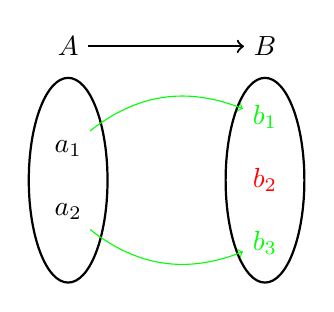
\begin{tikzpicture}
                \draw[thick] (0, 0.8) ellipse (0.5 and 1.3);
                \draw[thick] (2.5, 0.8) ellipse (0.5 and 1.3);

                \node (A1) at (0,1.2) {$a_1$};
                \node (A2) at (0,0.4) {$a_2$};

                \node (B1) at (2.5,1.6) {\green{$b_1$}};
                \node (B2) at (2.5,0.8) {\red{$b_2$}};
                \node (B3) at (2.5,0) {\green{$b_3$}};

                \node (A) at (0,2.5) {$A$};
                \node (B) at (2.5,2.5) {$B$};

                \draw[thick, ->] (A) -- (B);
                \draw[green, ->, bend left] (A1) to (B1);
                \draw[green, ->, bend right] (A2) to (B3);
            \end{tikzpicture}
        \end{minipage}
        \begin{minipage}{4cm}
            \parbox{4cm}{Die Abbildung \\ist \green{injektiv},\\aber \red{nicht surjektiv}}
        \end{minipage}

        \gray{"Höchstens ein Pfeil zeigt auf jedes Element in B" $\implies$ injektiv}
        \mesk
        \item \red{surjektiv}, falls $\forall b \in B \; \exists a \in A: b = f(a)$, d.h. $f[A] = B$
        \smsk

        \begin{minipage}{5cm}
            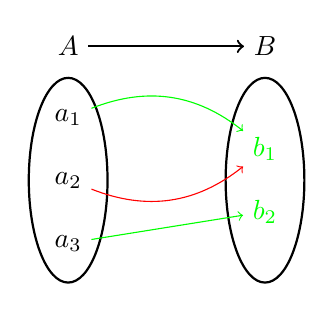
\begin{tikzpicture}
                \draw[thick] (0, 0.8) ellipse (0.5 and 1.3);
                \draw[thick] (2.5, 0.8) ellipse (0.5 and 1.3);

                \node (A1) at (0,1.6) {$a_1$};
                \node (A2) at (0,0.8) {$a_2$};
                \node (A3) at (0,0) {$a_3$};

                \node (B1) at (2.5,1.2) {\green{$b_1$}};
                \node (B2) at (2.5,0.4) {\green{$b_2$}};

                \node (A) at (0,2.5) {$A$};
                \node (B) at (2.5,2.5) {$B$};

                \draw[thick, ->] (A) -- (B);
                \draw[green, ->, bend left] (A1) to (B1);
                \draw[red, ->, bend right] (A2) to (B1);
                \draw[green, ->] (A3) -- (B2);
            \end{tikzpicture}
        \end{minipage}
        \begin{minipage}{4cm}
            \parbox{4cm}{Die Abbildung \\ist \green{surjektiv},\\aber \red{nicht injektiv}}
        \end{minipage}

        \gray{"Zu jedem Element in B geht ein Pfeil" $\implies$ surjektiv}
        \mesk
        \item \red{bijektiv}, falls $\forall b \in B \; \exists! a \in A: b = f(a)$
        \smsk

        \begin{minipage}{5cm}
            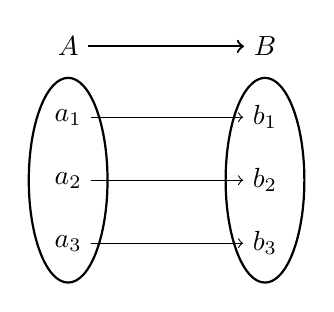
\begin{tikzpicture}
                \draw[thick] (0, 0.8) ellipse (0.5 and 1.3);
                \draw[thick] (2.5, 0.8) ellipse (0.5 and 1.3);

                \node (A1) at (0,1.6) {$a_1$};
                \node (A2) at (0,0.8) {$a_2$};
                \node (A3) at (0,0) {$a_3$};

                \node (B1) at (2.5,1.6) {$b_1$};
                \node (B2) at (2.5,0.8) {$b_2$};
                \node (B3) at (2.5,0) {$b_3$};

                \node (A) at (0,2.5) {$A$};
                \node (B) at (2.5,2.5) {$B$};

                \draw[thick, ->] (A) -- (B);
                \draw[->] (A1) -- (B1);
                \draw[->] (A2) -- (B2);
                \draw[->] (A3) -- (B3);
            \end{tikzpicture}
        \end{minipage}
        \begin{minipage}{4cm}
            \parbox{4cm}{Die Abbildung ist \\\green{bijektiv}, also sowohl \\injektiv als auch surjektiv}
        \end{minipage}

    \end{itemize}
}

\ex $f: \R \to \R, x \mapsto x^2$
\begin{itemize}
    \item $f$ ist nicht injektiv, da $f(-1) = f(1) = 1$\\
    \gray{Somit zeigen zwei Elemente $x \in A$ auf das gleiche Element $y \in B$}
    \item $f$ ist nicht surjektiv, da $f(x) \geq 0 \; \forall x \in R$\\
    \gray{Negative Werte in B werden nicht abgebildet $\implies$ nicht surjektiv}
\end{itemize}

\subsubsection{Umkehrabbildung}
\de{Die \red{Umkehrabbildung} einer Abbildung ist
    \begin{itemize}
        \item $f^{-1}: B \to A$, falls die Abbildung \red{bijektiv} ist
        \item $f^{-1}: f[A] \to A, b \mapsto a$ mit $f(a) = b$, falls die Abbildung \red{injektiv} ist
        \item allgemein für $B' \subseteq B$: $f^{-1}[B'] := \{a \in A \vst f(a) \in B'\} \subseteq A$\\
        \gray{In $B'$ sind alle Elemente aus B, die durch maximal ein Element in A abgebildet werden.}
    \end{itemize}
}

\subsubsection{Komposition von Abbildungen}

\de{Seien $f: a \to B$ und $g: B \to C$ Abbildungen, so ist die \red{Komposition} von f und g als die Abbildung $g \circ f: A \to C, \; a \mapsto g(f(a))$ definiert}
\begin{center}
    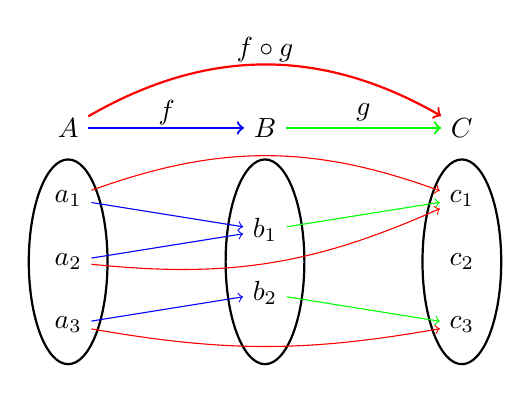
\begin{tikzpicture}
        \node (A) at (0,2.5) {$A$};
        \node (B) at (2.5,2.5) {$B$};
        \node (C) at (5,2.5) {$C$};
        \draw[thick] (0, 0.8) ellipse (0.5 and 1.3);
        \draw[thick] (2.5, 0.8) ellipse (0.5 and 1.3);
        \draw[thick] (5, 0.8) ellipse (0.5 and 1.3);

        \draw[blue, thick, ->] (A) -- (B);
        \draw[green, thick, ->] (B) -- (C);
        \draw[red, thick, ->, bend left] (A) to (C);
        \node (A) at (1.25,2.7) {$f$};
        \node (A) at (3.75,2.7) {$g$};
        \node (A) at (2.5,3.5) {$f \circ g$};

        \node (A1) at (0,1.6) {$a_1$};
        \node (A2) at (0,0.8) {$a_2$};
        \node (A3) at (0,0) {$a_3$};
        \node (B1) at (2.5,1.2) {$b_1$};
        \node (B2) at (2.5,0.4) {$b_2$};
        \node (C1) at (5,1.6) {$c_1$};
        \node (C2) at (5,0.8) {$c_2$};
        \node (C3) at (5,0) {$c_3$};

        \draw[blue, ->] (A1) -- (B1);
        \draw[blue, ->] (A2) -- (B1);
        \draw[blue, ->] (A3) -- (B2);
        \draw[green, ->] (B1) -- (C1);
        \draw[green, ->] (B2) -- (C3);
        \draw[red, ->, bend left=20] (A1) to (C1);
        \draw[red, ->, bend right=15] (A2) to (C1);
        \draw[red, ->, bend right=10] (A3) to (C3);
    \end{tikzpicture}
\end{center}

Bei der Mehrfachanwendung einer Abbildung gilt:\\
\gray{Die Potenz gibt an, wie oft die Abbildung angewendet wird}
\smsk

\begin{minipage}{4cm}
    \begin{itemize}
        \item $f^0: a \to A, \; a \mapsto a$
        \item $f^1: A \to A, \; f^1 \mapsto a$
        \item $f^2 := f \circ f$
    \end{itemize}
\end{minipage}
\begin{minipage}{7cm}
    \begin{itemize}
        \item $f^3 := f \circ f \circ f$
        \item $f^n := f^{n-1} \circ f = f \circ f^{n-1}$ für $n \geq 1$
    \end{itemize}
\end{minipage}

\newpage
\subsubsection{Identität von Abbildungen}

\de{Die Funktion $id_A: A \to A, a \mapsto a$ heißt \red{Identität von A}. Sie ist bijektiv und hat als einzige Abbildung die Eigenschaft, dass für jede Abbildung
\begin{itemize}
    \item $f: A \to B$ gilt: $f \circ id_A = f$
    \item $g: B \to A$ gilt: $id_A \circ g = g$
\end{itemize}
}
\gray{Die Identität ist das neutrale Element der Komposition und verändert nichts am Ergebnis: $f \circ id_A = id_A \circ f = f$}

\prop{Sei $A$ endlich und $f: A \to A$, Dann sind die folgenden äquivalent:
\begin{itemize}
    \item $f$ ist injektiv
    \item $f$ ist surjektiv
    \item $f$ ist bijektiv
\end{itemize}
}
\gray{Dies gilt nicht, wenn A unendlich ist. Zum Beispiel ist $f: \N \to \N, \; n \mapsto n + 1$ injektiv, nicht surjektiv, da es kein $n \in \N$ gibt, sodass $f(n) = 0$.\\
$f: \N \to \N, \; x \mapsto \begin{cases}
    x & \text{falls } x = 0\\
    x - 1 & \text{falls } x > 0\\
\end{cases}$
ist surjektiv, nicht injektiv, da $f(0) = f(1)$
}

\subsection{Größenvergleich von Mengen}

\de{Seien $A, B$ Mengen, so gilt
    \begin{itemize}
        \item $|A| = |B|$,falls es eine bijektive Abbildung $f: B \to A$ gibt
        \item $|A| \leq |B|$, falls es eine injektive Abbildung $f: A \to B$ gibt
        \item $|A| < |B|$, falls $|A| \leq |B|$ und $|A| \neq |B|$
    \end{itemize}
}

\ex \begin{itemize}
    \item $|\{1, 2, 3\}| = |\{*, \star, x\}|$

    \begin{minipage}{9.1cm}
        \item $|\N| = |\Z|$, denn $f: \N \to \Z, \; x \mapsto
        \begin{cases}
            \frac{x}{2} & \text{, falls } x \text{ gerade}\\
            -\frac{x + 1}{2} & \text{, falls } x \text{ ungerade}
        \end{cases}$
    \end{minipage}
    \begin{minipage}{2cm}
        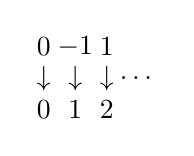
\begin{tikzpicture}
            \node at (0,0) {$0$};
            \node at (0,0.4) {$\downarrow$};
            \node at (0,0.8) {$0$};

            \node at (0.4,0) {$1$};
            \node at (0.4,0.4) {$\downarrow$};
            \node at (0.4,0.8) {$-1$};

            \node at (0.8,0) {$2$};
            \node at (0.8,0.4) {$\downarrow$};
            \node at (0.8,0.8) {$1$};

            \node at (1.2,0.4) {\dots};
        \end{tikzpicture}
    \end{minipage}
    \item $|\N| = |\N \times \N|$, denn $f: \N \times \N \to \N, \; f(x,y) = \frac{(x + y)^2 + 3 \cdot x + y}{2}$
\end{itemize}

\subsection{Der Satz von Cantor-Schröder-Bernstein}
\de{Der \red{Satz von Cantor} besagt, dass eine Menge $A$ immer weniger Elemente als ihre Potenzmenge $P(A)$ enthält.
\begin{equation*}
    |A| < |P(A)|
\end{equation*}
}
\pr{
    Spezialfall: $A = \emptyset$
    Dann ist $|A| = 0$ und $|P(A)| = |{\emptyset}| = 1$

    Sei $A \neq 0$:
    Wir zeigen zuerst "$\leq$". Sei $f: A \to P(A), \; a \mapsto \{a\}$, dann ist $f$ injektiv, also $|A| \leq |P(A)|$\\
    \gray{Da $P(A)$ für jedes Element $a \in A$ eine Menge $\{a\} \in P(A)$ enthält, kann hier das Element $a \in A$ auf $\{a\} \in P(A)$ abgebildet werden.}

    Jetzt zeigen wir "$\neq$": Wir müssen zeigen, dass eine injektive Abbildung $f: A \to P(A)$ niemals surjektiv ist.

    Sei $M := \{a \in A \vst a \notin P(A)\} \in P(a)$. Wir zeigen: $M \notin f[A]$

    Widerspruchsannahme: Sei $a \in A$ mit $f(a) = M$.

    Dann gilt, falls $a \in M$, dann $a \notin f(a) = M$ und falls $a \notin M$, dann $a \in f(a) =M$
}

\subsection{Das Auswahlaxiom}

\de{Das \red{Auswahlaxiom} besagt, dass es zu jeder nicht-leeren Menge S eine Auswahlabbildung $f$ gibt, die jeder Menge $X \in S$ ein Element $f(X) \in X$ zuordnet.}
\gray{Somit schafft das Auswahlaxiom die Möglichkeit "wähle eins aus", was innerhalb der ZF-Axiome nicht definiert ist.}

\de{Der \red{Unvollständigkeitssatz} besagt, dass mit ZF nicht gezeigt werden kann, dass ZF widerspruchsfrei ist.}

\subsection{Die Kontinuums-Hypothese}

\de{Die \red{Kontinuumshypothese} besagt, dass es keine Menge $M$ gibt, sodass $|\N| < |M| < |P(\N)|$ gilt.}
\gray{Die Kontinuumshypothese lässt sich weder beweisen, noch wiederlegen.}

\subsection{Permutationen}

\de{Eine \red{Permutation} ist eine bijektive Abbildung $\pi: X \to X$ einer endlichen Menge $X$. Die Menge aller Permutationen einer Menge mit $n$ Elementen heißt \red{$S_n$}}

Es gibt zwei gebräuchliche Schreibweisen für Permutationen:
\begin{itemize}
    \item
    \begin{tabular}{l r}
        $\pi =
        \begin{pmatrix}
            1 & 2 & \dots & n\\
            \pi(1) & \pi(2) & \dots & \pi(n)
        \end{pmatrix}$ &
        z.B. $\begin{pmatrix}
            1 & 2 & 3 & 4\\
            2 & 3 & 1 & 4
        \end{pmatrix}$
    \end{tabular}
    \item Zyklen-Schreibweise: $\pi = (1 \; 2 \; 3)(4) = (1 \; 2 \; 3)$, wobei Zyklen disjunkt sind
\end{itemize}
\begin{center}
    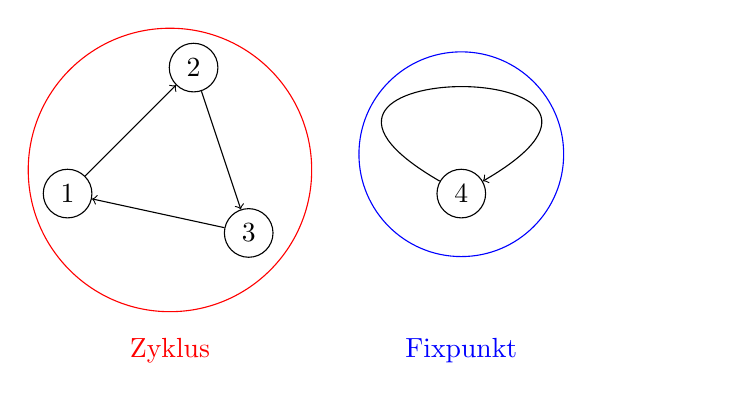
\begin{tikzpicture}
        \node[circle, draw] (1) at (0,1) {$1$};
        \node[circle, draw] (2) at (1.6,2.6) {$2$};
        \node[circle, draw] (3) at (2.3,0.5) {$3$};

        \draw[->,] (1) to (2);
        \draw[->,] (2) to (3);
        \draw[->,] (3) to (1);

        \node[circle, draw] (4) at (5, 1) {$4$};
        \draw[->, loop above, out=150, in=30, looseness=15] (4) to (4);

        \draw[red] (1.3,1.3) circle (1.8);
        \draw[blue] (5,1.5) circle (1.3);
        \node[red] at (1.3, -1) {Zyklus};
        \node[blue] at (5, -1) {Fixpunkt};
    \end{tikzpicture}
\end{center}

Allgemein:

Sei $\{x_{11}, x_{12}, \dots, x_{1j}, x_{21}, x_{22}, \dots, x_{2j}, \dots, x_{i1}, x_{i2}, \dots, x_{ij}\} \subseteq \{1, \dots, n\}$\\ mit allen $x_{ij}$ verschieden. Dann ist die Permutation $\pi$ definiert als:
\begin{equation*}
    \pi = \{x_{11}, x_{12}, \dots, x_{1j}\} \circ \{x_{21}, x_{22}, \dots, x_{2j}\} \circ \dots \circ \{x_{i1}, x_{i2}, \dots, x_{ij}\}
\end{equation*}
bedeutet:
\begin{center}
    \begin{minipage}{3cm}
        \begin{equation*}
            \begin{split}
                \pi(x_{11}) = x_{12}\\
                \pi(x_{21}) = x_{22}
            \end{split}
        \end{equation*}
    \end{minipage}
    \begin{minipage}{3cm}
        \begin{equation*}
            \begin{split}
                \pi(x_{12}) = x_{13}\\
                \pi(x_{22}) = x_{23}
            \end{split}
        \end{equation*}
    \end{minipage}
    \begin{minipage}{3cm}
        \begin{equation*}
            \begin{split}
                \dots\\
                \dots
            \end{split}
        \end{equation*}
    \end{minipage}
\end{center}

Diese Schreibweise ist nicht eindeutig, da
\begin{itemize}
    \item Zyklen vertauscht werden können:
    \begin{equation*}
        (1 \; 2) \; (3 \; 4) = (3 \; 4) \; (1 \; 2)
    \end{equation*}
    \item  Zyklen rotiert werden können, sodass ein beliebiges Element an erster Stelle steht:
    \begin{equation*}
        (1 \; 2 \; 3 \; 4) = (2 \; 3 \; 4 \; 1) = (3 \; 4 \; 1 \; 2) = (4 \; 1 \; 2 \; 3)
    \end{equation*}
    \item Zyklen der Länge, also Fixpunkte, ausgelassen werden können:
    \begin{equation*}
        (1 \; 2 \; 3) \; (4) = (1 \; 2 \; 3)
    \end{equation*}
\end{itemize}

\subsubsection{Komposition von Zyklen}
Es gibt 2 besondere Arten von Zyklen in Permutationen:
\begin{itemize}
    \item zyklische Permutationen: ein Zyklus der Länge $n$ in $S_n$
    \item Transposition: Zyklus der Länge $2$ $(ij) = (ji)$ mit $i \neq j$
\end{itemize}

Bei der Komposition von Zyklen gibt es mehrere Rechenregeln:
\begin{itemize}
    \item $(x_1 \; x_2 \; \dots \; x_i)^i = (1) = id_{\{1, 2, \dots, n\}}$\\
    \gray{Wenn also auf ein Element $x_i$ der Zyklus $i$-mal angewendet wird, ist das Ergebnis wieder das Element $x_i$}
    \item $(x_1 \; x_2 \; \dots \; x_i) \; (x_i \; x_{i+1} \; \dots \; x_{j}) = (x_1 \; x_2 \; \dots \; x_j)$ mit $\{x_1, x_2, \dots, x_j\} \subseteq \{1, 2, \dots, n\}$\\
    \ex $(1 \; 2 \; 3) \circ (3 \; 4 \; 5) = (1 \; 2 \; 3 \; 4 \; 5)$
\end{itemize}

\an{
    Wenn $(x_1 \; x_2 \; \dots \; x_k)$ und $(y_1 \; y_2 \; \dots \; y_l)$ disjunkte Zyklen sind, dann gilt:
    \begin{center}
        $(x_1 \; x_2 \; \dots \; x_k) \circ (y_1 \; y_2 \; \dots \; y_l) = (x_1 \; x_2 \; \dots \; x_k)(y_1 \; y_2 \; \dots \; y_l)$
    \end{center}
    Wenn die Zyklen nicht disjunkt sind, dann ist der zweite Ausdruck formal nicht korrekt, wird meist jedoch als Komposition angenommen.
}

\lem{
    Sei $(x_1 \; x_2 \; \dots \; x_k) \in S_n$ ein Zykel und $\pi \in S_n$. Dann gilt:
    \begin{equation*}
        \pi \circ (x_1 \; x_2 \; \dots \; x_k) \circ \pi^{-1} = (\pi(x_1) \; \pi(x_2) \; \dots \; \pi(x_k))
    \end{equation*}
}

\pr{
    Sei $\pi_i \in \{1, 2, \dots, n\}$. Jedes $j \in \{1, 2, \dots, n\}$ kann eindeutig so dargestellt werden:
    \begin{equation*}
        \begin{array}{lcl}
            \pi \circ \{x_1, ..., x_k\} \circ \pi^{-1}(\pi(i)) & = & \pi \circ \{x_1, ..., x_k\} \circ (i)\\
            & = &
            \begin{cases}
                \pi(x_{j+1}), \; i \notin \{x_1, ..., x_k\}\\
                \pi(x_l + 1), \; i = x_l\\
                \pi(x_1), \; i = x_k
            \end{cases}
        \end{array}
    \end{equation*}
}

\ex
\begin{equation*}
    \begin{array}{lcl}
        (1 \; 2) (3 \; 4 \; 5) \circ (2 \; 3) (1 \; 5) & = & (1 \; 2) (3 \; 4 \; 5) \circ (5 \; 1) (2 \; 3)\\
        & = & (1 \; 2) \circ (3 \; 4 \; 5 \; 1) \circ (2 \; 3)\\
        & = & (2 \; 1 \; 3 \; 4 \; 5) \circ (2 \; 3)\\
        & = & (4 \; 5 \; 2) \circ (2 \; 1 \; 3) \circ (2 \; 3)\\
        & = & (4 \; 5 \; 2)(1 \; 3) \circ (3 \; 2) \circ (3 \; 2)\\
        & = & (4 \; 5 \; 2)(1 \; 3)
    \end{array}
\end{equation*}

\prop{
    Jedes Element aus $S_n$ ist eine Komposition aus Zyklen.
}

\pr{
    Sei $(x_1 \dots x_k)$ ein Zyklus, dann gilt:
    \begin{equation*}
        (x_1 \dots x_k) = (x_1 \; x_2) \circ (x_2 \; x_3) \circ \dots \circ (x_{k-1} \; x_k)
    \end{equation*}
    Jedes $\pi \in S_n$ kann also als Komposition von Zyklen dargestellt werden.
}

\se{$|S_n| = n!$}

\pr{
    \begin{itemize}
        \item $n$ Möglichkeiten für $\pi(1)$
        \item $n-1$ Möglichkeiten für $\pi(2)$
        \item \dots
        \item $1$ Möglichkeit für $\pi(n)$
    \end{itemize}
}

\subsubsection{Stirlingsche Formel}

\se{
    \red{Stirlingsche Formel:} $\forall n \in \N: \sqrt{2 \pi n} \cdot (\frac{n}{e})^n < n! < \sqrt{2 \pi n} \cdot (\frac{n}{e})^n \cdot e^{\frac{1}{12n}}$\\
    $e = $ Eulersche Zahl $ = \sum_{k = 0}^{\infty}\frac{1}{k!} = 2,71728\dots$
}
\underline{Anwendung:} Wie viele Stellen hat 1000!?

Sei $lg$ der 10er-Logarithmus: $10^{lg(x)} = x$
\begin{equation*}
    \lg(\sqrt{1 \pi n} \cdot n^n \cdot (\frac{1}{e})^n) = \frac{1}{2} \cdot \lg(2 \pi n) + n \cdot \lg(n) - n \cdot \lg(e)
\end{equation*}
Für n = 1000: \red{$\approx 1,8991 + 3000 - 434,9448 = 2566,9543$}\\
Der "Fehlerterm", also die maximale Abweichung, beträgt $\lg(\frac{1}{e^{12n}}) \approx 0.00036$
$\implies 1000! \text{ hat } 2567 \text{ Stellen}$

\newpage
\section{Boolesche Funktionen und Aussagenlogik}

\subsection{Boolesche Funktionen}
\de{Sei $n \in N$. Eine (n-stellige) \red{Boolesche Funktion} ist eine Abbildung $f: \{0, 1\}^n \to \{0, 1\}$}
\an{
    $0$ wird aufgefasst als "falsch", $\perp$, F, F\\
    $1$ wird aufgefasst als "wahr", $\top$, T, W
}

\ex
\begin{itemize}
    \item Negationsfunktion: $\neg: \{0, 1\} \to \{0, 1\}, \begin{cases}
        \neg 0 = 1\\
        \neg 1 = 0
    \end{cases}$
    \item Konjunktion / UND: $\land: \{0, 1\}^2 \to \{0, 1\}, \begin{cases}
        0 \land 0 = 0\\
        0 \land 1 = 0\\
        1 \land 0 = 0\\
        1 \land 1 = 1
    \end{cases}$
    \item Disjunktion / ODER: $\lor: \{0, 1\}^2 \to \{0, 1\}, \begin{cases}
        0 \lor 0 = 0\\
        0 \lor 1 = 1\\
        1 \lor 0 = 1\\
        1 \lor 1 = 1
    \end{cases}$
\end{itemize}

\subsection{Rechengesetze}

$\forall x,y,z \in \{0, 1\}$ gilt:
\begin{equation*}
    \begin{array}{lcl}
        \text{Idempotenz} & x \land x = x & x \lor x = x\\
        \text{Kommutativität} & x \land y = y \land x & x \lor y = y \lor x\\
        \text{Assoziativität} & (x \land y) \land z = x \land (y \land z) & (x \lor y) \lor z = x \lor (y \lor z)\\
        \text{De-Morgansche Gesetze} & \neg(x \land y) = \neg x \lor \neg y & \neg(x \lor y) = \neg x \land \neg y
    \end{array}
\end{equation*}

Wir schreiben:
\begin{equation*}
    \begin{array}{lcl}
        x_1 \land x_2 \land \dots \land x_n & = & \bigwedge_{i = 1}^n x_i\\
        x_1 \lor x_2 \lor \dots \lor x_n & = & \bigvee_{i = 1}^n x_i
    \end{array}
\end{equation*}

\newpage
\subsection{Aussagenlogik}

\subsubsection{Syntax}

\de{Die \red{Syntax} behandelt Symbole und Regeln und wie sich diese Symbole zu Ausdrücken zusammenfügen lassen.}

\subsubsection{Ausdrücke}

\de{Ein \red{Ausdruck} besteht aus Variablensymbolen (z.B. $X,Y,Z,X_1,X_2$), Konnektoren (z.B. $\land, \lor, \neg$), $\perp$, $\top$ und Klammern. Klammern zeigen dabei nur eine Reihenfolge an.\\
\ex $X \land (\n{Y} \lor X) \land \top$

Ein \red{Ausdruck in den Variablen $S$}, wobei $S$ eine Menge ist, kann folgendermaßen rekursiv definiert werden:
\begin{itemize}
    \item Falls $X \in S_i$, dann ist $X$ ein Ausdruck
    \item $\top$ und $\perp$ sind Ausdrücke
    \item Falls $A$ ein Ausdruck ist, ist $\n{A}$ ein Ausdruck
    \item Falls $A_1$ und $A_2$ Ausdrücke sind, dann sind auch $(A_1 \land A_2)$ und $(A_1 \lor A_2)$ Ausdrücke
\end{itemize}
}

\ex X könnte stehen für:
\begin{itemize}
    \item $3 \cdot 2 = 6$ (wahr)
    \item $\emptyset \in \emptyset$ (falsch)
    \item $(3 \cdot 2 = 6) \land (\n{\emptyset \notin \emptyset})$ (falsch)
    \item $(3 \cdot 2 = 6) \lor (\emptyset \in \emptyset)$ (wahr)
\end{itemize}

\subsubsection{Semantik}

\de{Die \red{Semantik} behandelt die Bedeutung der Ausdrücke.}

\newpage
\subsubsection{Auswertungsfunktion}

\de{Sei $A$ ein Ausdruck in den Variablen $x_1, \dots, x_n$, dann ist die \red{Auswertungsfunktion} die n-stellige boolesche Operation $f_A: \{0, 1\}^n \to \{0, 1\}$ wie folgt:\\
Sei $(a_1, \dots, a_n) \in \{0, 1\}^n$, falls A die Gestalt
\begin{itemize}
    \item $X_i$ mit $i \in \{1, \dots, n\}$ hat, dann ist $f_A(a_1, \dots, a_n) := a_i$
    \item $\top$ hat, dann ist $f_A(a_1, \dots, a_n) := 1$
    \item $\perp$ hat, dann ist $f_A(a_1, \dots, a_n) := 0$
    \item $\n{B}$ hat, dann ist $f_A(a_1, \dots, a_n) = \n{f_B(a_1, \dots, a_n)}$
    \item $A_1 \land A_2$ für Ausdrücke $A_1, A_2$ hat, ist\\
    $f_A(a_y, \dots, a_n) = f_{A_1}(a_1, \dots, a_n) \land f_{A_2}(a_1, \dots, a_n)$
    \item $A_1 \lor A_2$ für Ausdrücke $A_1, A_2$ hat, ist\\
    $f_A(a_y, \dots, a_n) = f_{A_1}(a_1, \dots, a_n) \lor f_{A_2}(a_1, \dots, a_n)$
\end{itemize}
}

\subsubsection{Belegung eines ausdrucks}

\de{
    Eine Abbildung $\beta: S \to \{0, 1\}$ ist die \red{Belegung} der Variablen von S. Wir sagen: \red{$\beta$ erfüllt $A$}, falls $f_A(\beta(x_1), \dots, \beta(x_n)) = 1$\\
    Falls es eine Belegung gibt, die $A$ erfüllt, heißt $A$ erfüllbar, sonst unerfüllbar oder Kontradiktion.\\
    Falls jedes $\beta: S \to \{0, 1\}$ den Ausdruck $A$ erfüllt,, heißt $A$ \red{Tautologie}
}

\ex \begin{itemize}
    \item Der Ausdruck $X \land (\n{Y} \land Z)$ in den Variablen $X,Y,Z$ hat eine Belegung $(1, 0, 1)$
    \item Der Ausdruck $\top$ in den Variablen $X, Y$ ist eine Tautologie
    \item Der Ausdruck $X \lor \n{X}$ in den Variablen $X, Y$ ist eine Tautologie
    \item Der Ausdruck $X \land \n{X}$ in den Variablen $X, Y$ ist eine Kontradiktion
\end{itemize}

\an{Wir schreiben auch:}
\begin{equation*}
    \begin{array}{lclcl}
        \implies&:& \{0, 1\}^2 \to \{0, 1\} X \implies Y &:=& \n{X} \lor Y\\
        \iff&:& \{0, 1\}^2 \to \{0, 1\} X \iff Y &:=& (X \implies Y) \land (Y \implies X)
    \end{array}
\end{equation*}

Über $S$ definierte Ausdrücke $A$ und $B$ heißen äquivalent, wenn $A \iff B$ eine Tautologie ist. Das gilt genau dann, wenn $f_A = f_B$ gilt.

\newpage\ex
\begin{itemize}
    \item $X \land (\n{Y} \lor X)$ ist äquivalent zu $X$.\\
    Dies lässt sich mit dem Absorptionsgesetz zeigen: $X \land (X \lor \dots) = X$
    \item $X \implies Y$ ist äquivalent zu $\n{y} \implies \n{X}$
    \begin{equation*}
        \begin{array}{lcl}
            X \implies Y &\iff& \n{X} \lor Y\\
            &\iff& \n{\n{Y}} \lor \n{X}\\
            &\iff& \n{Y} \implies \n{X}
        \end{array}
    \end{equation*}
\end{itemize}

\subsubsection{Darstellungssatz}

\se{\red{Darstellungssatz}: Sei $f: \{0, 1\}^n \to \{0, 1\}$ eine boolesche Operation, dann gibt es einen aussagenlogischen Ausdruck $A$ mit $f = f_A$}
\pr{
    Definiere die Menge \( f^{-1}(1) \) als die Menge aller Tupel \( (b_1, \dots, b_n) \in \{0, 1\}^n \), für die \( f(b_1, \dots, b_n) = 1 \) gilt:
    \[
    f^{-1}(1) = \{(b_1, \dots, b_n) \in \{0, 1\}^n \mid f(b_1, \dots, b_n) = 1\}.
    \]

    Da \( f \) genau dann den Wert 1 annimmt, wenn eine der Belegungen in \( f^{-1}(1) \) vorliegt, können wir \( f(a_1, \dots, a_n) \) als eine Disjunktion über alle Elemente in \( f^{-1}(1) \) darstellen:
    \[
    f(a_1, \dots, a_n) = \bigvee_{(b_1, \dots, b_n) \in f^{-1}(1)} \left( \bigwedge_{b_i = 1} a_i \land \bigwedge_{b_i = 0} \n{a_i} \right).
    \]
    \[
    (a_1, \dots, a_n) = \bigwedge_{\{b_1, \dots, b_n\} \in f^{-1}(1)} (\bigwedge_{b_i = 1} (a_i) \land \bigwedge_{b_i = 0} (\n{a_i}))
    \]

    \gray{Hierbei gilt:
    \begin{itemize}
        \item Für jede Kombination \( (b_1, \dots, b_n) \in f^{-1}(1) \) konstruieren wir einen Konjunktionsterm, der \( a_i \) enthält, wenn \( b_i = 1 \), und \( \n{a_i} \), wenn \( b_i = 0 \).
        \item Diese Konjunktionsterme sind genau dann wahr, wenn die Belegung der Variablen \( (a_1, \dots, a_n) \) $\iff$ Kombination \( (b_1, \dots, b_n) \).
    \end{itemize}}
}

\newpage
\ex $(0 \; 0) \; (1 \; 0) \; (1 \; 1) = (\underbrace{\n{X} \land \n{Y}}_{(0 \; 0)}) \lor (\underbrace{X \land \n{Y}}_{(1 \; 0)}) \lor (\underbrace{X \land Y}_{(1 \; 1)})$

\subsubsection{Disjunkte Normalform}

\underline{Folgerung:} Jeder Ausdruck ist zu einem Ausdruck in \red{disjunkter Normalform (DNF)} äquivalent:
\[
    \bigvee_i \bigwedge_j l_{ij}, \text{ wobei } l_{ij} \begin{cases}
        \text{ eine Variable } (X_i) \to \text{"positives Literal"}\\
        \text{ eine negierte Variable } (\n{X_i}) \to \text{"negatives Literal"}
    \end{cases}
\]
\[
    \begin{array}{lcl}
        \bigvee_{\emptyset} = \perp & A \lor \bigvee_{\emptyset} \iff A
    \end{array}
\]
\gray{Eine Disjunkton ist genau dann wahr, wenn mindestens eine der vereinigten Aussagen wahr ist.}
\[
    \begin{array}{lcl}
        \bigwedge_{\emptyset} = \top & A \land \bigwedge_{\emptyset} \iff A
    \end{array}
\]
\gray{Eine Konjunktion ist genau dann falsch, wenn mindestens eine der konjugierten Aussagen falsch ist}

\an{
    In der Praxis benutzen wir oft:
    \begin{itemize}
        \item Ringschluss:
        \[
            (X_1 \implies X_2) \land (X_2 \implies X_3) \land \dots \land (X_n \implies X_1)
        \]
        ist äquivalent zu:
        \[
            \bigwedge_{(i,j) \in \{1, \dots, n\}^2} (X_i \iff X_j)
        \]
        \gray{Da sich alle Aussagen gegenseitig implizieren, sind alle Aussagen äquivalent, wenn der Ringschluss korrekt ist.}
        \item Kontraposition: \(X \implies Y\) ist äquivalent zu \(\n{Y} \implies \n{X}\)
        \item Widerspruchsbeweis: \((X \implies Y) \iff ((X \land \n{Y}) \implies \perp)\)
    \end{itemize}
}

\subsection{Erfüllbarkeitsproblem}

Das \red{Erfüllbarkeitsproblem} ist ein wichtiges Beispiel für ein Berechnungsproblem, bei dem ein aussagenlogischer Ausdruck gegeben und die Erfüllbarkeit von A herausgefunden werden soll.\\
Falls man alle Möglichkeiten für eine Belegung ausprobieren will, kommt man schon ab 185 Variablen auf mehr Fälle, als es Atome im beobachtbaren Universum gibt, da die Fälle exponentiell ($2^n$) steigen.

Es ist kein Verfahren bekannt, welches dieses Problem in polynomieller Zeit löst.\\
Als "P-NP-Problem" ist es eines der sieben Millennium-Probleme, für dessen Lösung eine Million Dollar Preisgeld ausgestellt werden.


Ein Spezialfall des Erfüllbarkeitsproblems ist die DNF:\\
Sei $A$ ein DNF: \(A_1 \lor A_2 \lor \dots \lor A_k\)
\begin{itemize}
    \item $A$ ist genau dann erfüllt, wenn eines der \(A_i \in \{1, \dots, k\}\) erfüllbar ist
    \item $A_i = l_{i1} \land \dots \land l_{ij}$ ist genau dann erfüllbar, wenn es keine zwei Literale \(l_{ij}, l_{ik}\) gibt, sodass \(l_{ij} = \n{l_{ik}}\)
\end{itemize}
Dieses Problem ist in polynomieller Zeit lösbar, allerdings ist es sehr ineffizient einen Ausdruck in DNF umzurechnen.

\subsubsection{konjunkte Normalform}

Ein anderer Spezialfall ist die Konjunktive Normalform (KNF):\\
Ein Ausdruck ist in KNF, falls er die Form
\[
    \bigwedge_i \underbrace{\bigvee_j \underbrace{l_{ij}}_{Literal}}_{Klausel}
\]
\gray{Wir betrachten Klauseln als Menge von Literalen.}

\lem{Jeder Ausdruck ist zu einem Ausdruck in konjunkter Normalform äquivalent.}
\pr{
    Sei $A$ ein Ausdruck und \(\n{A}\) in DNF: \(\bigvee_i \bigwedge_j l_{ij}\).\\
    Dann ist \(A \iff \n{\n{A}} \iff \n{\bigvee_i \bigwedge_j l_{ij}}\)\\
    Durch Umformung mit den De-Morganschen Gesetzen lässt sich der Ausdruck in KNF darstellen.\\
    \gray{Man erhält \(\bigwedge_i \bigvee_j \n{l_{ij}}\), was KNF ist.}
}

\newpage
\pr{
    Ein alternativer Beweisansatz funktioniert mithilfe des\\ Distributivgesetzes:\\
    \ex
    \[
        ((X_1 \land Y_1) \lor (x_2 \land Y_2) \lor \dots \lor (X_n \land Y_n)) \text{ (DNF)}
    \]
    \[
        \rightsquigarrow ((X_1 \land Y_1) \lor \dots \lor (X_n \land Y_n) \lor X_n) \land ((X_1 \land Y_1) \lor \dots \lor (X_n \land Y_n) \lor Y_n)
    \]
    \[\vdots\]
    \(2^n\) Konjunkte, d.h. \(2^n\) Klauseln.

    Es gilt: Wenn es für das Erfüllbarkeitsproblem in KNF einen\\
    polynomiellen Algorithmus gibt, dann auch für das allgemeine\\
    Erfüllbarkeitsproblem!
}

\subsection{Horn-SAT}

\subsubsection{Horn-Ausdrücke}

\de{
    Ein Ausdruck heißt \red{Horn}, falls jede Klausel höchstens ein positives Literal hat.\\
    \ex \underbar{X} $\land$ \underbar{U} $\land$ \underbar{$\n{Z}$} $\land$ \underbar{$(\n{X} \lor Y)$} $\land$ \underbar{$(\n{U} \lor \n{Y} \lor Z)$}\\
    Umformuliert: $X \land U \land \n{Z} \land (X \implies Y) \land ((U \land Y) \implies Z)$

    \begin{minipage}{2.2cm}
        \phantom{}
    \end{minipage}
    \begin{minipage}{1cm}
        $X = 1$\\
        $U = 1$
    \end{minipage}
    \begin{minipage}{1.3cm}
        $Z = 0$
    \end{minipage}
    \begin{minipage}{2.9cm}
        $Y = 1$
    \end{minipage}
    \begin{minipage}{1cm}
        \red{$Z = 1$}
    \end{minipage}

    Nicht erfüllbar!
}

\subsubsection{Lösungsalgorithmus}

Algorithmus für Horn-SAT (SAT = Erfüllbarkeitsproblem):
\begin{enumerate}
    \item Suche alle Klauseln der Gestalt $\{X\}$ und lösche $\n{X}$ in allen Klauseln
    \item Falls es jetzt eine LEERE Klausel gibt: nicht erfüllbar
    \item Gehe zu 1, bis keine Klausel der Form \(\{X\}\) vorhanden ist
    \item ERFÜLLBAR!
\end{enumerate}
Erfüllende Belegung: Alle Variablen mit Klausel \(\{X\}\) auf $1$, alle anderen auf $0$

\newpage
\ex \begin{itemize}
    \item $\{\underbar{X}\}$, $\{\underbar{U}\}$, $\{$\sout{$\n{Z}$}$\}$, $\{$\sout{$\n{X}$}, \underbar{Y}$\}$, $\{$\sout{$\n{U}$},\sout{$\n{Y}$},\underbar{$Z$}$\}$
\end{itemize}
Da die zweite Klausel leer ist, ist es nicht erfüllbar.

Falls $\beta$ eine Erfüllende Bedingung von $A$ ist, dann auch vom Ausdruck nach Schritt 1.\\
Umgekehrt: Die Belegung in Schritt 4 ist erfüllend, denn:
\begin{itemize}
    \item Alle Klauseln der Form $\{X\}$ sind wahr nach Konstruktion
    \item Alle anderen haben mindestens ein $\n{Y}$, und sind deshalb wahr
\end{itemize}

\an{
    Schritte 1 und 2 werden höchstens so oft durchlaufen, wie es Vaiablen gibt.\\
    Die Laufzeit ist "polynomiell", d.h. "effizient"
}


\section{Die natürlichen Zahlen}
\phantomsection
\addcontentsline{toc}{subsection}{\hspace{11cm}}
\subsubsection{Wohlordnung der natürlichen Zahlen}

\de{
    Für eine Menge $M$ sei $M^+ := M \cup \{M\} \mathrel{\reflectbox{$\subset$}} M$
    \[
        \begin{array}{lcl}
            0 &:=& \emptyset\\
            1 &:=& 0^+ = \emptyset \cup \{\emptyset\} = \{\emptyset\}\\
            2 &:=& 1^+ = \{\emptyset\} \cup \{\{\emptyset\}\} = \{\emptyset, \{\emptyset\}\}\\
            3 &:=& 2^+ = \{\emptyset, \{\emptyset\}\} \cup \{\{\emptyset, \{\emptyset\}\}\} = \{\emptyset, \{\emptyset\}, \{\emptyset, \{\emptyset\}\}\}\\
            n+1 &:=& n^+
        \end{array}
    \]
}

\subsubsection{Rechenoperationen}

Addition ist folgendermaßen induktiv definiert:
\[
    +: \N \times \N \to \N, n + 0 = n \text{ und } n + m^+ = (n + m)^+
\]
Subtraktion ist nur eine partielle Funktion:
\[
    - := \{(n, m) \in \N \times \N \vst n >= m\} \to \N, n - m := d \text{ mit } m + d = n
\]
Multiplikation:
\[
    \cdot: \N \times \N \to \N, n \cdot 0 = 0 \text{ und } n \cdot m^+ = n \cdot m + n
\]

Es gelten die bekannten Kommutativität-, Assoziativität- und \\Distributivitätsgesetze.

\[
    \N = \{0, 1, 2, 3, \dots\}
\]
Es gilt: Sei A eine Menge mit $0 \in A$. Falls $\forall a \in A, a^+ \in A$, dann ist $\N \subset A$. Dabei ist $\N$ das kleinste solche A.

Auf $\N$ gibt es eine Ordnung:
\[
    \begin{array}{lcl}
        n < m &\text{ falls }& n \in m \text{ oder } n \subset m\\
        n \leq m &\text{ falls }& n \subseteq m
    \end{array}
\]

\subsubsection{Ordnungen}

\de{
    Sei $A$ eine Menge. Eine \red{Ordnung} ist $R \subseteq A \times A$\\
    mit\begin{enumerate}
        \item $\forall a \in A: (a, a) \in R$
        \item $((a, b) \in R \land (b, c) \in R) \implies (a, c) \in R$
        \item $((a,b) \in R \cap (b, a) \in R) \implies a = b$
    \end{enumerate}
    Dieses $\leq$ ist eine Ordnung:
    \begin{itemize}
        \item reflexiv: $\forall n \in \N: n \leq n$
        \item transitiv: $\forall n_1, n_2, n_3 \in \N: n_1 \leq n_2 \land n_2 \leq n_3 \implies n_1 \leq n_3$
        \item anti-symmetrisch:\\$\forall n_1, n_2 \in \N: n_1 \leq n_2 \land n_2 \leq n_1 \implies n_1 = n_2$
    \end{itemize}
    Diese Ordnung ist \red{total}: $\forall n_1, n_2 \in \N: n_1 \leq n_2 \lor n_2 \leq n_1$\\
    und eine \red{Wohlordnung}:\\ $\forall T \subseteq \N \text{ mit } T \neq \emptyset, \exists! min(T) \in T: \forall n \in T: min(T) \leq n$

    \gray{
        Jede nicht-leere Teilmenge $T$ von $\N$ hat ein kleinstes Element $min(T)$\\
        Statt $(3,5) \in \leq$ schreiben wir $3 \leq 5$
    }
}

\ex $\leq$ auf $\Z$ ist keine Wohlordnung, da $\Z$ kein kleinstes Element hat.

\newpage
\subsection{Vollständige Induktion}

Seien $A_0, A_1, \dots$ Aussagen.\\
Wir zeigen: $\forall n\in \N: A_n$ ist wahr.\\
Wir gehen wie folgt vor:
\begin{enumerate}
    \item Induktionsanfang (IA): $A_0$ gilt
    \item Induktionsschritt (IS): $\forall n \in \N: A_n \implies A_{n+1}$
    \item Induktionsschluss: $\forall n \in \N: A_n$ ist wahr
\end{enumerate}
Warum funktioniert das?

Sei $T = \{n \in \N \vst A_n \text{ wahr}\}$\\
IA: $0 \in T$\\
IS: $\forall n \in T: n^+ \in T$\\
Daher: $T = \N$

\ex Zu zeigen: \(\forall n \in \N: \sum_{i=0}^{n}i = 0+1+\dots+n = \frac{n \cdot (n+1)}{2}\)\\
$A_n$ ist die Aussage $\sum_{i = 0}^{n}i = \frac{n \cdot (n+1)}{2}$
\begin{enumerate}
    \item IA: $A_0$ ist wahr:
    \[
        \sum_{i = 0}^{0}i = 0 = \frac{0 \cdot (0 + 1)}{2} \smsp \checkmark
    \]
    Induktionsvoraussetzung (IV):
    \[
        \sum_{i = 0}^{n}i = \frac{n \cdot (n+1)}{2}
    \]
    \item IS:
    \[
        \sum_{i = 0}^{n + 1}i = (n+1) + \sum_{i = 0}^{n}i \overset{IV}{=} (n+1) + \frac{n \cdot (n+1)}{2} = \frac{(n+1) \cdot (n+2)}{2}
    \]
    \item \qed
\end{enumerate}

\cl{Jede ungerade Zhl ist gerade.}
\pr{
    IV: $A_n$: die n-te ungerade Zahl $2n + 1$ ist gerade.

    IS: die (n+1)-te ungerade Zahl $2 (n + 1) + 1 = (2n+1) + 2$\\
    $2n + 1$ ist nach IV gerade, also ist der gesamte Term gerade.
}\\
\red{
    Problem: Der Induktionsanfang fehlt! Wir hätten nachweisen müssen, das 1 gerade ist.
}

\newpage
\se{
    Seien $A,B$ Mengen mit $|A| = |B| < \infty$ und sei $f: A \to B$ eine Abbildung, dann gilt:
    \[
        f \text{ ist injektiv} \iff f \text{ ist surjektiv} \iff f \text{ ist bijektiv}
    \]
}
\pr{
    Vollständige Induktion:\\
    $A_n:$ Seien $A,B$ Mengen mit $|A| = |B| = n$, dann ist jedes injektive $f: A \to B$ auch surjektiv.\\
    A: $n = 0$, $A = B = \emptyset$ und die leere Funktion $\emptyset \to \emptyset$ ist surjektiv.

    IV: $f': A \bs \{a\} \to B \bs \{f(a)\}, f'(a') = f(a')$ ist bijektiv.

    IS: Seien $A,B$ Mengen mit $|A| = |B| = n+1 > 0$ und $f: A \to B$ injektiv.\\
    Sei $a \in A$. Ein solches $a$ existiert, da $A \neq \emptyset$

    $f$ injektiv $\implies \forall a' \in A$ mit $a' \neq \emptyset: f(a') \neq f(a)'$,\\
    \gray{Zwei Elemente aus A zeigen nicht auf das gleiche Element in B, da die Abbildung injektiv ist}

    d.h. $f': A \bs \{a\} \to B \bs \{f(a)\}, \; f'(a') = f(a')$ ist eine injektive Abbildung.\\
    \gray{Wir definieren eine neue Abbildung, über alle Element von $A$ und $B$, bis auf $a$ und $f(a)$}

    $|A\bs \{a\}| = |B \bs \{f(a)\}| = n$\\
    \gray{Die Mächtigkeit der Mengen $A,B$ ist von $n+1$ um $1$ gesunken, da wir ein Element ausschließen}

    Dann: $f[A] = f'[A \bs \{a\}] \cup f[\{a\}] = B \bs \{f(a)\} \cup f[\{a\}] = B$
}

\subsection{Teilbarkeit}

\de{
    Seien $a,b \in \N$. Wir sagen \red{a teilt b}, oder a ist ein \red{Teiler} von b, oder b ist ein \red{Vielfaches von a} und schreiben $a \vst b$, falls $\exists k \in \N: b = a \cdot k$
}

\ex
\begin{itemize}
    \item $\forall n \in \N: n \vst 0$
    \item Falls $0 \vst n$, dann $n = 0$\\
    \gray{Teilbarkeit ist etwas anderes als Division. Obwohl Teilbarkeit durch 0 definiert ist, ist Division durch 0 nicht definiert.}
    \item $\forall n \in \N: 1 \vst n$
\end{itemize}
Falls $a \vst b$, dann $\frac{b}{q} = k$ mit $a \cdot k = b$

\newpage

\an{
    $\vst$ ist eine Ordnung. Sie ist reflexiv, transitiv und anti-symmetrisch.\\
    Sie ist \underline{nicht} total, da z.B. $2 \nmid 3$ und $3 \nmid 2$
}

\lem{
    Sei $a, b_1, b_2 \in \N$ und $a \vst b_1$ und $a \vst b_2$, $b_1 \geq b_2$.\\
    Dann: $a \vst (b_1 + b_2)$ und $a \vst (b_1 - b_2)$
}
\pr{
    Sei $k_1, k_2 \in \N$ mit $b_i = ak_i$; für $i = 1,2$.

    Dann gilt nach dem Distributivgesetz:
    \[
        \begin{array}{lclcl}
            (b_1 + b_2) &=& a \cdot k_1 + a \cdot k_2 &=& a \cdot (k_1 + k_2)\\
            (b_1 - b_2) &=& a \cdot k_1 - a \cdot k_2 &=& a \cdot (k_1 - k_2)
        \end{array}
    \]
}

\subsection{Primzahlen}

\de{
    Eine Zahl $p \in \N$ heißt \red{Primzahl}, falls $p \neq 1$ und\\
    $(a \vst p \land a \neq 1) \implies a = p$
}
\ex $2,3,5,7,11,13,17,19,23,29,31,37,\dots$

\se{Euklid: Es gibt unendlich viele Primzahlen}
\pr{
    Nehme an, es gäbe nur endlich viele Primzahlen $p_1, \dots, p_k$.\\
    Sei $n := \prod_{i=1}^{k}p_i + 1$

    \lem{
        $\exists i \in \{1,\dots,k\}$ mit $p_i \vst n$
    }
    \lem{
        $p_i \vst (n - \prod_{i=1}^{k}p_i)$, d.h. $p_i \vst n$
    }
    \red{Widerspruch!}
}

\newpage
\ex Teilbarkeitsdiagramm für $60$:
\begin{center}
    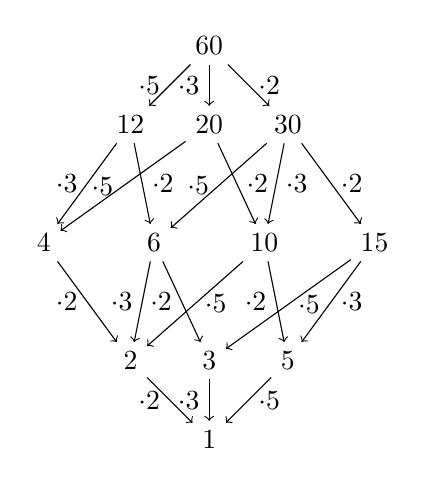
\begin{tikzpicture}
        \node (1) at (0,0) {1};

        \node (2) at (-1,1) {2};
        \node (3) at (0,1) {3};
        \node (5) at (1,1) {5};

        \node (4) at (-2.1,2.5) {4};
        \node (6) at (-0.7,2.5) {6};
        \node (10) at (0.7,2.5) {10};
        \node (15) at (2.1,2.5) {15};

        \node (12) at (-1, 4) {12};
        \node (20) at (0, 4) {20};
        \node (30) at (1, 4) {30};

        \node (60) at (0, 5) {60};

        \draw[->] (2) -- (1) node[midway, left] {$\cdot 2$};
        \draw[->] (3) -- (1) node[midway, left] {$\cdot 3$};
        \draw[->] (5) -- (1) node[midway, right] {$\cdot 5$};

        \draw[->] (4) -- (2) node[midway, left] {$\cdot 2$};
        \draw[->] (6) -- (2) node[midway, left] {$\cdot 3$};
        \draw[->] (6) -- (3) node[midway, left] {$\cdot 2$};
        \draw[->] (10) -- (2) node[midway, right] {$\cdot 5$};
        \draw[->] (10) -- (5) node[midway, left] {$\cdot 2$};
        \draw[->] (15) -- (3) node[midway, right] {$\cdot 5$};
        \draw[->] (15) -- (5) node[midway, right] {$\cdot 3$};

        \draw[->] (12) -- (4) node[midway, left] {$\cdot 3$};
        \draw[->] (12) -- (6) node[midway, right] {$\cdot 2$};
        \draw[->] (20) -- (4) node[midway, left] {$\cdot 5$};
        \draw[->] (20) -- (10) node[midway, right] {$\cdot 2$};
        \draw[->] (30) -- (6) node[midway, left] {$\cdot 5$};
        \draw[->] (30) -- (10) node[midway, right] {$\cdot 3$};
        \draw[->] (30) -- (15) node[midway, right] {$\cdot 2$};

        \draw[->] (60) -- (12) node[midway, left] {$\cdot 5$};
        \draw[->] (60) -- (20) node[midway, left] {$\cdot 3$};
        \draw[->] (60) -- (30) node[midway, right] {$\cdot 2$};
    \end{tikzpicture}
\end{center}

\an{
    Sei $\pi(n)$ die Anzahl der Primzahlen $\leq n$. Es gibt eine "asymptotische Abschätzung" für $\pi(n)$, der Primzahlsatz:
    \[
        \pi(n) \sim \frac{n}{\ln(n)}
    \]
    d.h.
    \[
        \forall \varepsilon > 0, \exists n_0 \in \N: \forall n > n_0: \; \vline \frac{\pi(n) \cdot \ln(n)}{n} -1 \; \vline < \varepsilon
    \]
}

\underline{Offene Frage:} Gibt es unendlich viele Primzahlen $p$, für die $p + 2$ eine Primzahl ist?

Primzahlen sind die "Elementarbausteine" der natürlichen Zahlen.

\subsubsection{Fundamentalsatz der Arithmetik}

\red{Fundamentalsatz der Arithmetik:}
\begin{quote}
    Sei $n \in \N, \; n > 0$.\\
    Dann $\exists! k \in \N$ und $\exists! p_1,\dots,p_k \in \N$ Primzahlen mit $p_1 < \dots < p_k$ und $\exists! \alpha_1, \dots, \alpha_k \in \N \bs \{0\}: n = \prod_{i = 1}^{k} p_i^{\alpha_i} = p_1^{\alpha_1} \cdot \dots \cdot p_k^{\alpha_k}$
\end{quote}

\ex \begin{itemize}
    \item $n = 60; k = 3; p_1 = 2, p_2 = 3, p_3 = 5; \alpha_1 = 2, \alpha_2 = 1, \alpha_3 = 1$\\
    $60 = 2^2 \cdot 3^1 \cdot 5^1$
    \item $n = 1; k = 0; 1 = \prod_{i = 1}^{0} p_i^{a_i}$ "leeres Produkt"
\end{itemize}

\newpage
\de{
    Die ganzen Zahlen $\Z$ sind folgendermaßen definiert:
    \[
        \Z := \{0, 1, -1, 2, -2, 3, -3, \dots\}
    \]
    d.h.
    \[
        z \in \Z: |z| := \begin{cases}
            z & \text{ falls } z \in \N\\
            -z & \text{ falls } z \notin \N
        \end{cases}
    \]
    Außerdem: $a \vst b$ falls $\exists k \in \Z, \; a \cdot k = b$\\
    \ex $-3 \vst 6$ da $-3 \cdot (-2) = 6$
}

\subsection{Der euklidische Algorithmus}

\de{
    Seien $a,b \in \N$. Der \red{größte gemeinsame Teiler} (ggT) von $a$ und $b$ ist die größte Zahl $d \in \N$ mit $d \st a$ und $d \st b$, geschrieben $d = ggT(a,b)$ und $ggT(0,0) := 0$
}

\lem{
    Division mit Rest: Seien $a, b \in \Z, \; b \neq 0$.\\
    Dann $\exists! q,r \in \Z$ mit $a = q \cdot b + r$ und $0 \leq r < b$
}

\pr{
    Falls $b > 0$:\\
    Beweis für die Existenz:\\
    Sei $q \in \Z$ größtmöglich mit $b \cdot q \leq a$\\
    Setze $r := a - b \cdot q$, dann ist $r \geq 0$\\
    Außerdem ist $b \cdot (q+1) > 0$, also:
    \[
        r = a - b \cdot q < b \cdot (q+1) - b \cdot q < b
    \]
    Eindeutigkeit: Sei $a = q \cdot b + r = q' \cdot b + r'$ mit $q, q' \in \Z$ und $0 \leq r,r' < b$\\
    Ohne Beschränkung der Allgemeinheit (O.B.d.A.): $q' \geq q$\\
    Dann: $b \cdot (q - q') = r' - r$, also $b \cdot \underbrace{(q' - q)}_{\geq 0} + r' = r < b$\\
    Falls $q' > q$ ist $b \cdot (q' - q) + r' \geq b$ \red{Wiederspruch!}\\
    Also gilt $q = q'$ und $r = r'$

    Falls $b < 0$ müssen einige Vorzeichen vertauscht werden, allerdings bleibt die Beweismethode gleich.
}

\red{Notation:} Wir schreiben $a$ mod $b = r$

\prop{
    Seien $a,b \in \N$ mit $b > 0$.\\
    Dann: $ggT(a,b) = ggT(a, a \text{ mod } b)$
}
\pr{
    Sei $a = q \cdot b + r$.
    Sei $d := ggT(a,b)$ und $d' := ggT(b,r)$

    $d \st a$ und $d \st b \implies d \st \underbrace{(a - b \cdot q)}_r$, also $d \leq d'$\\
    \gray{Da $d$ Teiler von $b$ und $r$ und $d'$ der ggT von $b$ und $r$, muss $d \leq d'$}

    $d' \st b$ und $d' \st r \implies d' \st \underbrace{(b \cdot q + r)}_a$, also $d' \leq d$\\
    \gray{Wie oben folgt hieraus analog $d' \leq d$}

    $\implies d' = d$
}

\red{Euklidischer Algorithmus:} EUKLID$(m,n)$
\begin{quote}
    \underline{Eingabe:} $m,n \in \N$ mit $m \leq n$\\
    Falls $m = 0$: Gebe $n$ aus.\\
    Sonst: Gebe EUKLID$(n \text{ mod } m, m)$ aus.

    \underline{Ausgabe} ist ggT$(m,n)$
\end{quote}

\subsubsection{Lemma von Bézout}

\co{
    \red{Lemma von Bézout:} Sei $m,n \in \N$. Dann gibt es $a, b \in \Z$ mit $ggT(m,n) = a \cdot m + b \cdot n$
}

\pr{
    Mit vollständiger Induktion:\\
    \underline{$A_k$:} $\forall m,n \in \{0, \dots, k\} \smsp \exists a,b \in \Z: ggT(m,n) = a \cdot m + b \cdot n$

    \underline{$IA$:} $k = 0, \; m = n = 0, \; 0 = 0 \cdot 0 + 0 \cdot 0$

    \underline{$IS$:} Seien $m,n \in \{0, \dots, k+1\}$\\
    Falls $m = n$: $m = n = ggT(m,n)$ und $m = 1 \cdot m + 0 \cdot n$

    Falls $m \neq n$, O.B.d.A. $m < n$\\
    Seien $q,r \in \N$ mit $r < m$ und $n = q \cdot m + r$\\
    Dann: $ggT(m,n) = ggT(r, m) \overset{IV}{=} (\exists a',b' \in \Z:) a' \cdot r + b' \cdot m$

    Dann setze: $a := b' - a' \cdot q$ und $b := a'$\\
    Dann gilt: $a \cdot m + b \cdot n = (b' - a' \cdot q) \cdot m + a' \cdot (q \cdot m + r) = a' \cdot r + b' \cdot m = ggT(m,n)$
}

\subsubsection{Erweiterter Euklidischer Algorithmus}

\red{Erweiterter Euklidischer Algorithmus:} E-EUKLID$(m,n)$
\begin{quote}
    \underline{Eingabe:} $m,n \in \N$ mit $m \leq n$\\
    \underline{Ausgabe:} $a, b \in \Z$ mit $ggT(m,n) = a \cdot m + b \cdot n$

    Falls $m \st n$: Gebe $(1,0)$ aus.

    Sonst: Berechne $q, r \in \N$ mit $r < m$ und $n = q \cdot m + r$\\
    Sei $(a',b')$ die Ausgabe von E-EUKLID$(r,m)$.\\
    Gebe $(b' - a' \cdot q, b')$ aus.
\end{quote}

\subsubsection{Euklids Lemma}

\lem{
    \red{Euklids Lemma}

    Sei $p$ eine Primzahl. Dann gilt: $p \st a \cdot b \implies p \st a \lor p \st b$
}
\pr{
    Angenommen $p \st mn$, aber $p \nmid m$.

    Es ist zu zeigen, dass $p \st n$:\\
    $ggT(n,p) = 1$.\\
    Nach Bezout:\\
    $\exists a,b \in \Z: a \cdot p + b \cdot n = 1$ $\st \cdot m$\\
    $p \cdot (am) + (nm) \cdot b = m$

    Es gilt: $p \st p(am)$ und nach Vorraussetzung/Implikation $p \st mn$

    Analog für $p \nmid n$
}

\lem{Jede natürliche Zahl, außer Null, hat eine Primfaktorzerlegung: Sei $n \in \N, \; n \neq 1$. Dann $\exists p \in \N, \; p \text{ prim mit } p \vst n$}
\newpage
\pr{
    Sei $A \subseteq \N: A:= \{n \in \N \vst n > 1 \land \nexists p \text{ prim}: p \vst n\}$

    \gray{Wir leiten einen Widerspruchsbeweis ein.}\\
    Annahme: $A \neq \emptyset$.

    Dann hat $A$ ein kleinstes Element $a$. $a$ ist keine Primzahl, denn $a \vst a$.\\
    \gray{Das ist so, da es dann nicht in der Menge $A$ enthalten wäre.}

    Also $\exists b \in \N$ mit $1 < b < a$ und $b \vst a$.\\
    \gray{Jede Zahl, die keine Primzahl ist, hat einen Teiler.}

    $a$ minimal $\implies \exists \text{ Primzahl } p: p \vst b$.\\
    Dann gilt: $p \vst a$ - \red{Wiederspruch!}\\
    \gray{Gegenteilig zu den Vorraussetzungen durch die Menge. Somit muss die Menge leer sein.}
}

Die Primfaktorzerlegung ist eindeutig:

$n \in N \bs \{0\}$\\
Primfaktorzerlegung von $n$: $\prod_{i = 1}^{r}p_1^{a_i} \quad p_1 < \dots < p_r, p_1, \dots, p_r$ sind Primzahlen\\
Primfaktorzerlegung von $1$: $\prod_{i = 1}^{\emptyset}p_1^{a_i} = 1$ (leeres Produkt)

\pr{
    (Widerspruchsbeweis)\\
    Angenommen es gibt ein $n \in \N \bs \{0\}$ mit zwei verschiedenen Primfaktorzerlegungen $Z_1, Z_2$. Wähle $n$ kleinstmöglich.\\
    Nach dem Lemma von Euklid teilt jeder Primfaktor $p$ von $Z_1$ auch einen Primfaktor $q$ von $Z_2$\\
    \gray{Entweder $p$ teilt $q$ oder $p$ teilt $Z_2/q$, in welchem Falls das ganze für $Z_2/q$ getestet werden kann.}\\
    Deshalb gilt: $p=q$\\
    \gray{Da $p$ und $q$ beides Primzhalen sind, müssen sie gleich sein.}

    Dann: $Z_1/p$ und $Z_2/p$ sind zwei verschiedene Primfaktorzerlegungen von $n/p$.\\
    Dies würde bedeuten, dass $n/p = n/q$ zwei verschiedene Primfaktorzerlegungen hat, was jedoch ein Widerspruch zur Minimalität von $n$ nach der Annahme ist.

    Also gilt: $Z_1 = Z_2$
}

\newpage
\subsubsection{Chinesischer Restsatz}
\se{
    Seien $m,n$ teilerfremd mit $k,l \in \N$.\\
    Dann gibt es genau ein $x \in \{0, \dots, m \cdot n - 1\}$\\
    mit \begin{enumerate}
        \item $x \mod m = k \mod m$ bzw. $x \equiv k \mod m$
        \item $x \mod n = l \mod n$ bzw. $x \equiv l \mod n$
    \end{enumerate}
}
\pr{
    Nach Bezout: $\exists a,b \in \Z: am + bn = 1$

    $x := l \cdot am + k \cdot bn$
    \begin{align*}
        lam + kbn &\equiv kbn \mesp (\text{mod } m) \mesp \text{\gray{Da $lam$ ein Vielfaches von $m$ ist}}\\
        &\equiv (1 - am) \cdot k \mesp (\text{mod } m) \mesp \text{\gray{Umstellen obere Gleichung}}\\
        &\equiv k \mesp (\text{mod } m) \mesp \text{\gray{Da $-amk$ ein Vielfaches von m ist}}\\
    \end{align*}
    Analog für $n$:
    \[
        lam + kbn \equiv l \cdot am \equiv (1-bn) \cdot l \equiv l \mesp (\text{mod } n)
    \]
}

\section{Modulare Arithmetik}

\subsection{Modulorechnung}

\de{
    Sei $A$ eine Menge.\\
    Eine Operation $A^k$ nach $A$ heißt ($k$-stellige) \red{Operation auf $A$}
}
$\Z_n = \{0, 1, \dots, n-1\}$
Definierte auf $\Z_n$ eine zweistellige Operation $\oplus$ und eine zweistellige Operation $\odot$:
\[
    \begin{array}{lcl}
        a \oplus b &:=& (a + b) \mod n\\
        a \odot b &:=& (a \cdot b) \mod n
    \end{array}
\]

Für $n = 3$:
\begin{center}
    \begin{minipage}{3.7cm}
        \begin{tabular}{c|c|c|c}
            $\oplus$ & 0 & 1 & 2\\
            \hline
            0 & 0 & 1 & 2\\
            1 & 1 & 2 & 0\\
            2 & 2 & 0 & 1
        \end{tabular}
    \end{minipage}
    \begin{minipage}{2.7cm}
        \begin{tabular}{c|c|c|c}
            $\odot$ & 0 & 1 & 2\\
            \hline
            0 & 0 & 0 & 0\\
            1 & 0 & 1 & 2\\
            2 & 0 & 2 & 1
        \end{tabular}
    \end{minipage}
\end{center}

\subsection{Homomorphieregel}

\[
    \begin{array}{lcl}
        (a + b) \mod n &=& (a \mod n) \oplus (b \mod n)\\
        (a \cdot b) \mod n &=& (a \mod n) \odot (b \mod n)
    \end{array}
\]

\subsubsection{Al Kashi's Trick}

\an{Wie lässt sich $a^b \mod c$ berechnen?}
\begin{enumerate}
    \item Binäre Exponentiation
    \item Homomorphieregel
\end{enumerate}
\ex \begin{itemize}
    \item $x^4 = x \cdot x \cdot x \cdot x = (x^2)^2$
    \item $x^{11} = \left( \left( x^2 \right)^2 \right)^2 \cdot x^2 \cdot x$
\end{itemize}
"Quadrieren und Multiplizieren"

\begin{enumerate}
    \item Schreibe den Exponenten in Binär:\\
    $n = 11 = 1 \cdot 8 + 0 \cdot 4 + 1 \cdot 2 + 1 \cdot 1 \implies 1011$
    \item Starte mit x
    \item Falls nächste Ziffer 0: Quadrieren
    \item Falls nächste Ziffer 1: Quadrieren und mit x multiplizieren
\end{enumerate}

Warum funktioniert das?
\[
    \forall b \in \N \; \exists q \in \N: a^b = a^{2q+r} = a^{2q} \cdot a^r \text{ mit } r \in \{0,1\}
\]
lässt sich rekursiv mit $b = 2q$ anwenden

\ex $2^{100000} \mod 100001$\\
$100000 = 2^{16} + 2^{15} + 2^{10} + 2^9 + 2^7 + 2^5$\\
Binär: $1100001101010000$

$\left( 2^2 \cdot 2\right)^{(2 \cdot 2 \cdot 2 \cdot 2) \cdot 2} \dots$\\
Zwischenergebnisse Modulo $100001$ berechnen

\subsection{Entscheidungsprobleme}

\begin{itemize}
    \item $a,b \in \N$. Was ist $a \cdot b$?\\
    Mit Schulmathematik polynomiell lösbar.
    \item Division mit Rest (Modulo):\\
    $a,b \in \N$ mit $b \neq 0$. Was ist $a \mod b$?\\
    Mit Schulmathematik polynomiell lösbar.
    \item Primzahl-Test:\\
    $n \in \N$. Ist $n$ eine Primzahl?\\
    \underline{2002:} "Primes is in P" $\implies$ polynomiell lösbar
    \item geg: $n \in \N$ und $i \in \N$. Ist das $i$-te Bit des größten Primfaktors von $n$ eine $1$?\\
    Kein polynomielles Verfahren bekannt
    \item geg: aussagenlogische Formel. Ist die Formel erfüllbar?\\
    Vermutlich existiert kein polynomielles Verfahren
\end{itemize}

\newpage
\section{Gruppen}

\de{
    Eine \red{Gruppe} besteht aus
    \begin{itemize}
        \item einer Menge $G$ von Elementen
        \item einer zweistellige Operation auf $G$, d.h.: $f: G^2 \to G$ ("Gruppenoperation")
        \item einer einstelligen Operation $^{-1}: G \to G$ ("Inversenbildung")
        \item dem neutralen Element $e \in G$
    \end{itemize}
    mit den folgenden Eigenschaften:
    \begin{itemize}
        \item Assoziativität: $\forall a,b,c \in G: a \cdot (b \cdot c) = (a \cdot b) \cdot c$
        \item neutrales Element: $\forall a \in G: a \cdot e = e \cdot a = a$
        \item Inversenbildung: $\forall a \in G: a \cdot a^{-1} = a^{-1} \cdot a = e$
    \end{itemize}
}
\ex \begin{itemize}
    \item $(\Z,+,-,0)$
    \item $\Q$
    \item $\R$
    \item $\C$
    \item $(\Z_n, \oplus, \ominus, 0)$
\end{itemize}

\subsection{\texorpdfstring{Die multiplikative Gruppe $\Z_n$}{Die multiplikative Gruppe Z}}

$\Z_n = \{0, \dots, n - 1\} \subseteq \Z$\\
mit $\cdot: \Z_n^2 \to \Z_n: (x,y) \mapsto (x \cdot y) \mod n$
\begin{itemize}
    \item ist assoziativ \checkmark
    \item neutrales Element 1
    \item Inverses Element: $x \cdot x^{-1} \equiv x^{-1} \cdot x \equiv 1 \; (\mod n)$
\end{itemize}

$Z_6 = \{0,1,2,3,4,5\}$

\underline{Angenommen}, $2$ hat Inverses: $2 \cdot x \equiv 1 (\mod 6)$

$2 \cdot i \equiv 1 (\mod 6)$

$3 \equiv 3 \cdot 1 \equiv 3 \cdot (2 \cdot i) \equiv \frac{3 \cdot 2}{0} (\mod 6)$ \red{Wiederspruch!}

\subsubsection{Nullteiler}
\de{
    Mann nennt $a \in \Z_n \bs \{0\}$ \red{Nullteiler}, wenn es ein $b \in \Z_n \bs \{0\}$ gibt, mit $a \cdot b = 0$
}
\ex $2$ ist ein Nullteiler in $\Z_6$, da $2 \cdot 3 = 0 \; (\mod 6)$

\subsubsection{Einheiten}
\de{Ein Element $a \in \Z_n$ heißt \red{Einheit}, falls es ein $b \in \Z_n$ gibt mit $a \cdot b = 1$}

\de{
    Die Menge aller Einheiten in $\Z_n$ ist die \red{Einheitsgruppe} $\Z_n^*$
}

\ex Einheiten in $\Z_6$ sind $5, 1$.

\lem{
    Sei $m \in \Z_n \bs \{0\}$.
    Dann sind äquivalent:
    \begin{itemize}
        \item $m$ ist Einheit in $\Z_n$.
        \item $m$ ist kein Nullteiler
        \item $m,n$ sind teilerfremd: $ggT(m,n) = 1$
    \end{itemize}
}
\pr{
    $1 \implies 2$ Wiederspruchsbeweis:\\
    Sei $m$ ein Nullteiler in $\Z_n \bs \{0\}$, d.h. $\exists b \in \Z_n \bs \{0\}: m \cdot b = 0$\\
    Angenommen, $m$ ist eine Einheit, d.h. $\exists i \in \Z_n: m \cdot i = 1$

    \[
        0 = i \cdot 0 = i \cdot (m \cdot b) = (i \cdot m) \cdot b = b \text{\red{\quad Wiederspruch!}}
    \]

    $2 \implies 3$ Beweis der Kontraposition: $\n{3} \implies \n{2}$:

    Angenommen, $ggT(m,n) > 1$\\
    Zu zeigen: $m$ ist Nullteiler:
    \[
        m' := \frac{n}{ggT(m,n)} \in \Z_n \bs \{0\}
    \]
    $m \cdot m'$ ist ein Vielfaches von n, also $m \cdot m' \equiv 0 \; (\mod n)$

    Zu zeigen bleibt: $\forall a,b \in Z_n$ ist $a \cdot b \in \Z$:\\
    das Inverse von $a \cdot b$ ist $(a \cdot b)^{-1} = a^{-1} \cdot b^{-1}$
}

\subsubsection{\texorpdfstring{Die eulersche $\varphi$-Funktion}{Die eulersche phi-Funktion}}

\de{
    Die \red{eulersche $\varphi$-Funktion} $\varphi(n)$ beschreibt die Anzahl der Einheiten der multiplikativen Gruppe:
    $$\varphi(n) = |\Z_n^*|$$
    Falls $n$ eine Primzahl ist, so gilt: $\varphi(n) = n - 1$.\\
    Falls $n$ die Potenz einer Primzahl $p^k$ ist, so gilt: $\varphi(n) = p^{k-1} \cdot (p-1)$

    \gray{Alle Zahlen, die nicht teilerfremd zu $p^k$ sind:\\
    $p, p^2, \dots, p^k$ ($\frac{p^k}{k}$ Zahlen)}
}

\lem{
    Seien $n,m$ Primzahlen. Dann gilt: $\varphi(m \cdot n) = \varphi(n) \cdot \varphi(m)$
}

\pr{
    Sei $f: \Z_{nm} \to \Z_n \times \Z_m: f(a) = (a \mod n, a \mod m)$.\\
    Diese Abbildung ist nach dem chinesischen Restsatz bijektiv.\\
    Es gilt: $\ggt(a,nm) = 1 \iff \ggt(a,m) = 1$\\
    \gray{(Beweis analog mit $\ggt(a,n) = 1$)}

    Deshalb gibt es eine Umkehrfunktion $\Z_{mn}^* = f^{-1}(\Z_n^* \cdot \Z_m^*)$ und es gilt:
    \[
        \varphi(nm) = |\Z_n^* \cdot \Z_m^*| = |\Z_n^*| \cdot |\Z_m^*| = \varphi(n) \cdot \varphi(m)
    \]
}\\
\co{
    Sei $n = p_1^{\alpha_1} \cdot \dots \cdot p_k^{\alpha_k}$ in Primfaktorzerlegung.\\
    Dann gilt: $\varphi(n) = \varphi(p_1^{\alpha_1}) \cdot \dots \cdot \varphi(p_k^{\alpha_k})$
}

\subsection{Zyklische Gruppen}

\subsubsection{Permutationsgruppen}
\de{
    \red{Permutationsgruppen:} Sei $X$ eine Menge. Sym$(X)$ ist die Menge aller Permutationen auf $X$.
    Es wird eine Gruppe bezüglich
    \begin{itemize}
        \item der Komposition $\circ$ als Gruppenoperation.
        \item dem neutralen Element $id_X$ für alle $\pi \in$ Sym$(X)$: $\pi \circ id_X = id_X \circ \pi = \pi$
        \item dem Inversen Element, die Umkehrfunktion $\pi^{-1}$
    \end{itemize}
}

\subsubsection{Abelsche Gruppen}
\de{
    Alle diese Gruppen sind \red{abelsch}, d.h. die Gruppenoperation ist kommutativ: $\forall a,b \in G: a \cdot b = b \cdot a$
}

Schreibweise: $(G, \cdot, ^{-1}, e)$\\
Häufig auch: $(G, \cdot)$

$e$ und $g^{-1}$ sind ($\forall g \in G$) bereits eindeutig durch $\cdot$ festgelegt.

$\pi_1 \circ \pi_2 = \begin{pmatrix}
    1 & 2 & 3\\
    3 & 2 & 1
\end{pmatrix}$


$|x| > 2$, dann ist Sym$(x)$ \underline{nicht} abelsch:

$\pi_1 = \begin{pmatrix}
    1 & 2 & 3\\
    2 & 3 & 1
\end{pmatrix}
= (1 \; 2 \; 3)$

$\pi_2 = \begin{pmatrix}
    1 & 2 & 3\\
    2 & 1 & 3
\end{pmatrix}
= (1 \; 2) \; (3)$

\subsubsection{Erzeuger}
\de{
    Eine Gruppe $(G; *)$ heißt \red{zyklisch}, wenn es ein $g \in G$ gibt, sodass
    $$G = \{e, g^1, g^{-1}, g \circ g, (g \circ g)^{-2}, ...\} = \{g^n \vst n \in \Z\}$$
    Die Zahl $g$ heißt \red{Erzeuger} von $G$.
}

\ex \begin{itemize}
    \item Erzeuger von $(\Z; +)$ ist $1$
    \item Erzeuger von $(\Z_n; +)$ ist $1$
\end{itemize}

\subsubsection{Isomorphismen}
\de{
    Gruppen $(G, *)$ und $(H, \cdot)$ heißen \red{isomorph}, falls es eine Bijektion $f: G \to H$ gibt, sodass gilt:
    $$f(a \circ b) = f(a) \cdot f(b)$$
    Diese Abbildung ist ein \red{Gruppenisomorphismus}.
}

\newpage
\prop{
    Sei $(G; *)$ eine zyklische Gruppe mit dem Erzeuger $g$.

    Wenn $G$ unendlich ist, dann ist: $f: \Z \to G: k \mapsto gk$ ein Gruppenisomorphismus.\\
    Sonst sei $|G| = n \in \N$. Dann ist $f: \Z_n \to G: k \mapsto g^k$ ein Gruppenisomorphismus.
}

\pr{
    $f(k + l) = g^{k+l} = g^k + g^l$ in beiden Fällen.

    Beweis der Injektivität, Surjektivität folgt in beiden Fällen:

    1. Fall: $G$ ist unendlich.\\
    Falls $k-l = n \ne 0$, dann ist $g^m = g^{m \mod n}$ \red{Widerspruch!}\\
    \gray{$g^m$ kann sich nicht wiederholen, da die Menge unendlich ist}

    2. Fall: $G$ ist endlich. Es gibt ein kleinstes $g^m = e$.\\
    Damit hat $G = \{e,g,g^2,\dots,g^m-1\}$ die Kardinalität $m$.
}

\prop{
    Jede Primzahl $p < n$ ist ein Erzeuger in $\Z_n$. Somit ist die Anzahl der Erzeuger $= \varphi(n)$
}

\pr{
    Falls $d = \ggt(a,n) > 1$, dann ist $a, 2a, \dots$ immer durch $d$ teilbar, also ist $1 \notin \{a,2a,\dots\}$ und ist kein Erzeuger von $\Z_n$.

    Falls $\ggt(a,n) = 1$, dann gibt es nach dem Lemma von Bezout:
    \begin{align*}
        k,l \in \Z&: 1 = ka + ln\\
        \text{Für } b \in \Z_n&: b = b \cdot ka + \underbrace{b \cdot ln }_{\mod n = 0}\text{ und } \underbrace{b = a + a + \dots + a}_{b \cdot k-Mal}
    \end{align*}
}

\de{
    Falls $(\Z_n^*)$ zyklisch ist, dan heißt ein Erzeuger von $\Z_n^*$ \red{Primitivwurzel}.
}

\an{
    Wenn $n$ eine Primzahl ist, dann ist $Z_n^*$ zyklisch ist, und es gibt $\varphi(\varphi(n))$ Primitivwurzeln.
}

\newpage
\ex $T_{12}^* = \{1,3,7,11\}$ ist nicht zyklisch:
\begin{itemize}
    \item $1 \cdot 1 \equiv 1$ (mod $12$)
    \item $5 \cdot 5 \equiv 25 \equiv 1$ (mod $12$)
    \item $7 \cdot 7 \equiv 49 \equiv 1$ (mod $12$)
    \item $11 \cdot 11 \equiv 121 \equiv 1$ (mod $12$)x
\end{itemize}

\subsection{Der diskrete Logarithmus}

Sei $p$ eine Primzahl und $g$ eine Primitiv-Wurzel von $\Z_p^*$, also $\Z_p^*$ zyklisch.\\
Dann ist $\exp_g: Z_{p-1} \to \Z_p^*: k \mapsto g^k$ ein Isomorphismus.

\de{
    Der \red{diskrete Logarithmus} zur Basis $g$ ist definiert als die\\
    Umkehrfunktion von $\exp_g$:
    \[
        \log_g: \Z_p^* \to \Z_{p-1}: a \mapsto k \text{ mit } g^k \equiv a \; (\mod p)
    \]
}

Zur Lösung des diskreten Logarithmus ist kein Algorithmus in polynomieller Laufzeit bekannt:

Eingabe: Primzahl $p$, Primitiv-Wurzel $g$, $a \in \Z_p^*$\\
Ausgabe: $log_x(a) \in \Z_{p-1}$

Deshalb wird $\exp_p$ auch Einbahnfunktion genannt.\\
Eine weitere Einbahnfunktion ist die Faktorisierung von $n = p \cdot q$ mit Primzahlen $p,q$.

Beides sind Grundlagen für Verschlüsselungstechniken.

\subsubsection{Beispiel: Diffie-Hellmann-Merkle-Verfahren}

Es wird öffentlich eine Primzahl $p$ und eine Primitiv-Wurzel $g$ aus $\Z_p^*$ gewählt.

\blue{Person 1 wählt eine zufällige Zahl $a \in \Z_{p-1}$ und berechnet $a' = g^a \mod p$}\\
\red{Person 2 wählt eine zufällige Zahl $b \in \Z_{p-1}$ und berechnet $b' = g^b \mod p$}

$a'$ und $b'$ werden öffentlich ausgetauscht.

\blue{Person 1 berechnet $c \equiv (b')^a \equiv g^{b \cdot a} \;(\mod p)$}\\
\red{Person 2 berechnet $c \equiv (a')^b \equiv g^{a \cdot b} \;(\mod p)$}

Mithilfe von $c$ können jetzt Nachrichten verschlüsselt werden:

Sei $m = \{m_1, \dots, m_l\}$ eine Nachricht mit $m_i \in \Z_2$ (Binärdarstellung)\\
Sei $c_1,\dots,c_k$ die Binärschreibweise von $c$, wobei $k \geq l$ (sonst teile $m$ in mehrere Nachrichten)

Die verschlüsselte Nachricht hat die Form\\
$V := (c_1 + m_1 \mod 2, \dots, c_l + m_l \mod 2)$\\
Die entschlüsselte Nachricht hat die Form \\
$(m_1, \dots, m_l) = (c_1 + (c_1 + m_1 \mod 2), \dots, c_l + (c_l + m_l \mod 2))$

\subsection{Untergruppen}

\de{
    Sei $(G; *)$ eine Gruppe. Eine \red{Untergruppe} $U$ von $G$ ist eine Teilemenge $U \subseteq G$, sodass $(U, *)$ eine Gruppe ist.

    explizit: $e \in U$ und $\forall g,h \in U: g \cdot h, g^{-1} \in U$
}

\ex \begin{itemize}
    \item $\{x \in \Z \st x \text{ gerade}\}$ ist Untergruppe von $(\Z; +)$
    \item $\Z, \Q$ sind Untergruppen von $\R$
    \item $\{(1 \; 2), id\}$ ist Untergruppe von $S_n$
\end{itemize}

\de{
    Sei $(G; *)$ eine Gruppe und $g \in G$. Dann ist die von $g$ erzeugte Untergruppen die kleinste Untergruppe $\spann{g}$ von $G$, die $g$ enthält.

    explizit: $\spann{g} = \{g^k \mid k \in \Z\}$
}

\ex $\spann{\emptyset} = \{e\}$ ist die triviale Untergruppe

\subsubsection{Ordnungen}

\de{
    Sei $(G; *)$ eine Gruppe. Die \red{Ordnung} von $G$ ist $|G|$.\\
    Sei $g \in G$. Die Ordnung von $g$ ist $|\spann{g}|$
}

\ex \begin{itemize}
    \item Wenn $(x_1 \; \dots \; x_n)$ ein $k$-Zyklus in $S_n$ ist, dann ist die Ordnung von $(x_1 \; \dots \; x_k)$ gleich k
    \item Die Ordnung von $2$ in $\Z$ ist unendlich
    \item Wenn $g$ eine Primitiv-Wurzel mod $p$ prim ist, dann ist die Ordnung von $g$ gleich $p-1$
    \item Sei ein Element von $S_n$: $\sigma = (x_1 \; \dots \; x_k) \; (y_1 \; \dots \; y_l)$ in Zyklenschreibweise, dann ist die Ordnung von $\sigma$ das kleinste gemeinsame Vielfache von $k$ und $l$
\end{itemize}

\an{
    Sei $G$ eine Gruppe mit $g \in G$. Dann gilt:
    \[
        |\spann{g}| = \min\{n \in \N \bs \{0\} \st g^n = e\}
    \]
    Denn: $g^k = g^{k \mod(ord(g))}$ \gray{$ord(g)$ ist die Ordnung von $g$}
}

\subsubsection{Nebenklassen}

\de{
    Sei $G$ eine Gruppe und $U$ eine Untergruppe von $G$. Sei $g \in G$.\\
    Dann ist $g \circ U := \{g \circ U \st u \in U\}$ die \red{Linksnebenklasse}.\\
    Analog ist $U \circ g := \{u \circ g \st u \in U\}$ die \red{Rechtsnebenklasse}.
}

\ex $(\R^n; +), v \in \R^n, U \in \R^n$ ist UVR. Dann ist $v + U$ der affine Teilraum von $\R^n$; Nebenklassen sind genau affine Teilräume.

\an{
    Jedes $g \in G$ ist in einer Nebenklasse enthalten, nämlich in $g \circ U$, denn $e \in U$.\\
    \gray{Mit jedem $g \in G$ lässt sich mit $U$ eine Nebenklasse bilden, da $e \in U$. Siehe affine Teilräume}
}

\an{
    Die Abbildung $U \to g \circ U: u \mapsto g \circ u$ ist bijektiv.\\
    \pr{
        Surjektiv nach Definition von $g \circ U$.\\
        Seien $u_1, u_2 \in U$ mit $g \circ u_1 = g \circ u_2 \implies u_1 = u_2$, also injektiv.
    }\\
    Besonders: $|U| = |g \circ U| = |U \circ g|$
}

\lem{
    Zwei Nebenklassen $g \circ U$ und $h \circ U$ sind entweder gleich oder disjunkt.
}

\pr{
    \begin{enumerate}
        \item Falls $x \in c \circ U$, dann gilt: $x \circ U \subseteq c \circ U$\\
        Sei $u \in U$ und $a = g \circ u$. Dann gilt:
        \[
            g \circ u = (a \circ u^{-1}) \circ u = a \circ (u^{-1} \circ u) = a \circ e = a \in a \circ U
        \]
        \item Falls $x \circ U \subseteq c \circ U$, dann gilt: $x \circ U = c \circ U$
    \end{enumerate}

    Angenommen $g \circ U \cap h \circ U \ne \emptyset$:\\
    Sei $a \in g \circ U \cap h \circ U$, dann ist $a \in g \circ U$ und $a \in h \circ U$.\\
    Nach 1. und 2. gilt deshalb: $a \circ U = g \circ U$ und $a \circ U = h \circ U$.\\
    Somit gilt $g \circ U = h \circ U$
}

\subsubsection{Index von Nebenklassen}

\de{
    Sei $G$ eine Gruppe und $U$ eine Untergruppe von $G$. Der \red{Index} von $U$ in $G$ ist die Anzahl der Nebenklassen von $U$ in $G$ und wird mit $[G:U] = |\{g \circ U \st g \in G\}|$ bezeichnet.\\
    \gray{"Nebenklassen" bezieht sich hier auf Links- oder Rechts-\\
    nebenklassen, aber nicht auf alle zusammen}
}

\subsection{Satz von Lagrange}

\de{
    Sei $G$ eine endliche Gruppe, $U$ eine UG von $G$. Dann gilt:
    \[
        [G:U] = \frac{|G|}{|U|}
    \]
    Insbesondere: $|U|$ teilt $|G|$
}

\pr{
    $$G = \bigcup_{g \in G} g \circ U$$
    Das sind $[G:U]$-viele Nebenklassen der Kardinalität $|U| = |g \circ U|$
}

\co{
    Sei $G$ endlicm it $g \in G$.\\
    Dann ist  die Ordnung von $g$ ein Teiler von $|G|$ und $g^{|G|} = e$
}

\pr{
    $|\spann{g}| = |G|$ wegen Lagrange. Sei $|\spann{g}| = k$ und $k \cdot l = |G|$:
    \[
        g^{|G|} = g^{k \cdot l} = (g^k)^l = e^l = e
    \]
}

\ex \begin{itemize}
    \item $G \in \Z$, $n \in \N_+$. Dann ist $n \cdot \Z = \{n \cdot a | a \in \Z\}$ eine UG.\\
    Sei $b \in \Z$. Dann ist $b + n \cdot \Z = \{b + n \cdot a | a \in \Z\}$ eine Nebenklasse, d.h die Nebenklassen sind genau die Restklassen.

    Das ist die "übliche Definition von $\Z_n$:
    \[
        \Z_n = \Z \bs \{n \cdot \Z\} = \{a + n \cdot\}
    \]
    \item $G = D_4$, $u = \spann{r}$ \gray{$r$ ist die Rotation um $90$°}\\
    $|U| = 4$. Es gibt zwei Nebenklassen: Die Menge der Rotationen und die Menge der Spiegelungen.
\end{itemize}

\ex \begin{enumerate}
    \item "Kleiner Satz von Fermat": $a \in \Z_p$, $p$ teilt nicht $a$.\\
    Dann gilt: $a^{p-1} \equiv 1 \; (\mod p)$\\
    \pr{
        $a \mod p$ ist einheit in $Z_p^*$ und $|\Z_p^*| = p - 1$\\
        $\implies a^{p-1} \equiv 1 (\mod p)$
    }
    \item "Satz von Euler-Fernand": Sei $n \in \N$, $a \in \Z$ mit $\ggt(a,n) = 1$.\\
    Dann gilt: $a^{\varphi(n)} \equiv 1 \; (\mod n)$
    \pr{
        Analog zu oben mit $\varphi(n)$ statt $p-1$
    }
\end{enumerate}

\subsection{Das RSA-Verfahren}

\red{
    Bob:
    \begin{enumerate}
        \item Wählt zufällig zwei (große) Primzahlen $p,q$.
        \item Berechnet $n = p \cdot q$
        \item Wählt zufällig $d$ mit $\ggt(d, \varphi(n)) = 1$
        \item Berechnet $i = d^{-1} \in \Z_{\varphi(n)}^*$ (mit E-Euklid)
    \end{enumerate}
}
Der öffentliche Schlüssel ist $(n,d)$, er wird übertragen.\\
\blue{
    Alice:
    \begin{enumerate}
        \item Berechnet $c := m^i \mod n$ für die Nachricht mit $m \le n-1$
    \end{enumerate}
}
Die Nachricht $m$ wird öffentlich übertragen.

Dann: $c^d \equiv m^{i \cdot i} \equiv m^{1 + k \cdot \varphi(n)} \equiv m \cdot (m^{\varphi(n)})^k \equiv m \; (\mod n)$

Angriffsmöglichkeiten:
\begin{itemize}
    \item Wenn man $n = p \cdot q$ faktorisieren kann, lässt sich $\varphi(n)$ und damit auch $d/i$ berechnen.
    \item Durch geschicktes Erraten der Nachrichten (z.B "Ja") und deren Verschlüsselung kann der private Schlüssel herausgefunden werden.\\
    In der Praxis werden werden allerdings Zufallsbits angehängt, wodurch die Nachrichten nicht erraten werden können.
\end{itemize}

\ex RSA-Anwendung: Signieren

Damit Bob weiß, dass die Nachricht $m$ tatsächlich von Alice kommt, kann Alice diese signieren.

Sei $(m_A, i_A)$ der öffentliche Schlüssel und $d_A$ der private Schlüssel von Bob.\\
Alice verschickt $m_A$ und $s := m^{d_A} \mod n_A$.\\
Bob berechnet $s^{i_A} \mod n_A$

Dabei muss gelten: $s^{i_A} \equiv m^{d_Ai_A} \equiv m \mod n_A$

Das lässt sich kombinieren: erst verschlüsseln und dann signieren.

\ex Alice möchte Bob "I LOVE YOU" schicken.
\begin{enumerate}
    \item Schlüsselerstellung: B wählt $p = 59$ und $q = 71$.\\
    Dann berechnet er $n = 59 \cdot 71 = 4189$ und $\varphi(n) = (p-1) \cdot (q-1) = 58 \cdot 70 = 4060$\\
    B wählt $d$ teilerfremd zu $4060$, z.B $d = 13$ (\red{privater Schlüssel})

    Er berechnet $i \equiv 13^{-1} \; (\mod 4060)$ mit dem erweiterten euklidischen Algorithmus: $1 = -3 \cdot 4060 + 937 \cdot 13 \implies i = 937$
    \item Schlüsselübermittlung: B schickt $(n,i) = (4189,937)$ an A.
    \item Verschlüsselung: zuerst codiert A ihre Nachricht: $\text{Leer} = 00, A = 01, B = 02, \dots, J = 10, \dots$\\
    Aus "I LOVE YOU" wird $"090 012 152 205 002 515 21"$. Dies ist größer als $n$, also muss es in Pakete geteilt werden.

    Für jedes Paket (z.B $"090"$) berechnet A: $C := 90^{937} \mod 4189 = 998$ mit Al-Kashi.
    \item Nachrichtenübermittlung: A schickt $998$ und die anderen verschlüsselten Pakete an B.
    \item Entschlüsselung: B berechnet für alle Pakte: $998^13 \equiv 90 (\mod 4189)$ und hat somit "I LOVE YOU" entschlüsselt.
\end{enumerate}

\newpage
\section{Graphen}

\an{
    Schleifen sind nicht erlaubt und Knoten dürfen nicht doppelt verbunden werden.
}

\an{
    Für eine Menge $M$ schreiben wir $\vvec{M}{2} := \{A \subseteq M \st |A| = 2\}$, die Menge aller zweielementigen Teilmengen von $M$.

    Falls $M$ endlich ist: $|\vvec{M}{2}| = \vvec{|M|}{2} = \frac{|M| \cdot (|M| - 1)}{2}$
}

\de{
    Ein Graph ist ein Paar $G=(V(G), E(G))$ mit
    \begin{itemize}
        \item $V(G)$ eine Menge ("Knotenmenge")
        \item $E(G) \subseteq \vvec{V(G)}{2}$ ("Kantenmenge")
    \end{itemize}
}

Wenn der Graph aus dem Kontext geschlossen werden kann, schreiben wir auch nur $G = (V,E)$.\\
Diese Graphen heißen schlicht bzw. einfach und ungerichtet.

\ex \begin{itemize}
    \item Knoten: Facebook-Profile\\
    Kanten: $\{a,b\} \in E$, falls $a,b$ befreundet sind
    \item Knoten: Schauspieler\\
    Kanten: $\{a,b\} \in E$, falls es einen film gibt, in dem beide mitspielen
\end{itemize}

\phantomsection
\addcontentsline{toc}{subsection}{\hspace{11cm}}
\subsubsection{Wichtige Beispiele für Graphen}

\begin{itemize}
    \item $n \in \N, \red{K_n := (V,E)}$, wobei $V = \{1, \dots, n\}$ und $E = \vvec{V}{2}$, heißt\\
    \red{$n$-elementige Clique} oder \red{$n$-elementiger vollständiger Graph}
    \item $\red{I_n := (\{1, \dots, n\}, \emptyset)}$ ist die \red{stabile Menge} der Größe $n$
    \item $\red{P_n := (\{1, \dots, n\}, \{\{1,2\}, \{2,3\}, \dots, \{n-1,n\}\})}$ ist der \red{Pfad} der Länge $n \ge 2$
    \item $\red{C_n := (\{1, \dots, n\}, \{\{1,2\}, \{2,3\}, \dots, \{n-1,n\}, \{n,1\}\})}$ ist der \red{Kreis} der Länge $n \ge 3$
\end{itemize}

\subsubsection{Adjazente Knoten}

\an{
    Wenn $\{u,v\} \in E$, dann heißen $u,w$ \red{benachbart} oder \red{adjazent}. \\
    Der \red{Grad} von $v$ ist die Anzahl seiner Nachbarn.
}

\ex In $P_5$ haben $1,5$ den Grad $1$ und $2,3,4$ den Grad $2$.

\de{
    Sei $G = (V,E)$ ein Graph. Der \red{Komplementärgraph} von $G$ ist $$\n{G} := (V, \vvec{V}{2} \bs \{E\})$$
}

\an{
    $\n{\n{G}} = G$ und $\n{K_n} = I_n$
}

\subsubsection{isomorphisme Graphen}

\de{
    Seien $G,H$ Graphen. ein \red{Isomorphismus} von $G$ nach $H$ ist eine Bijektion $f: V(G) \to V(H)$ mit\\
    $\{u,v\} \in E(G) \iff \{f(u), f(v)\} \in E(H)$.\\
    Dann sind $G,H$ isomorph.
}

\ex Ein Isomorphismus von $C_5$ nach $\n{C_5}$ lautet:
$$f \in S_n, f = \begin{pmatrix}
    1 & 2 & 3 & 4 & 5\\
    1 & 3 & 5 & 2 & 4
\end{pmatrix}$$

\subsubsection{Subgraphen}

\de{
    Seien $G,H$ Graphen. $H$ heißt
    \begin{itemize}
        \item \red{Supgraph} von $G$,falls $V(H) \subseteq V(G)$ und $E(H \subseteq E(G))$
        \item \red{induzierter Subgraph} von $G$, falls $V(H) \subseteq V(G)$\\
        und $E(H) = \vvec{V(H)}{2} \cap E(G)$
        Dann ist $H$ durch $G$ und $V(H)$ eindeutig definiert und wir schreiben $H = G[V(H)]$
    \end{itemize}
}

\newpage
\ex \begin{itemize}
    \item $P_3, C_3$ sind Subgraphen von $K_5$
    \item $C_3$ ist induzierter Subgraph von $K_5$
    \item $K_4$ ist induzierter Subgraph von $K_5$
    \item $P_5$ ist Subgraph von $C_5$, aber kein induzierter Subgraph
\end{itemize}

\subsubsection{Kantenzüge}

\de{
    Sei $G=(V,E)$ ein Graph. Ein \red{Kantenzug} von $u_1$ nach $u_2$, wobei $u_1,u_2 \in V$, ist eine Kantenfolge $(u_1, \dots, u_l)$ mit $\{u_i, u_{i+1}\} \in E$ für alle $i \in \{1, \dots, l-1\}$

    Ein Kantenzug heißt \red{geschlossen}, falls $u_1 = u_l$, sonst heißt er \red{offen}\\
    Ein Kantenzug heißt \red{Weg} oder \red{Pfad}, falls alle Knoten des Kantenzuges verschieden sind\\
    Ein Kantenzug heißt \red{Kreis}, falls er geschlossen ist und $(u_1, \dots, u_{l-1})$ ein Weg ist
}

\subsection{Zusammenhängende Knoten}

\de{
    Ein Graph $G=V(,E)$ heißt \red{zusammenhängend}, falls es für je zwei $s,t \in V$ einen Kantenzug von $s$ nach $t$ gibt.
}

\an{
    Wenn es einen Kantenzug von $s$ nach $t$ gibt, dann auch einen Pfad:
    $$(s,u_1,\dots,u_l,t)$$
    ist ein Kantenzug. Für alle $u_i = u_j$ im Kantenzug, existiert dann ein Pfad:
    $$(s, u_1,\dots,u_i,u_{j+1},\dots,u_l,t)$$
}

\subsubsection{Die disjunkte Vereinigung}
\de{
    Seien $G,H$ Graphen mit $V(G) \cap V(H) = \emptyset$. Die \red{disjunkte Vereinigung} von $G,H$ ist:
    $$G \uplus H := (V(G) \cup V(H), E(G) \cup E(H))$$
}

\prop{
    Ein Graph $G=(V,E)$ mit $V \ne \emptyset$ ist genau dann zusammenhängend,\\
    falls er nicht als disjunkte Vereinigungen nzweier nicht leerer\\
     Graphen geschrieben werden kann, d.h:
    $$
        \forall V_1, v_2 \subseteq V; V_1,V_2 \ne \emptyset; V_1 \cap V_2 = \emptyset: G \ne G[V_1] \uplus G(V_2)
    $$
}

\pr{
    \underline{Richtung $\implies$}: Seien $V_1, V_2 \subseteq V; V_1,V_2 \ne \emptyset; V_1 \cap V_2 = \emptyset$\\
    Angenommen $G = G[V_1] \uplus G(V_2)$:

    Dann ist $G$ zusammenhängend und es gibt einen Kantenzug\\
    $(u,u_1,...,u_l,v)$

    Sei $i$ der Index des ersten Elements mit $u_i \in V_2$.\\
    Dann ist $\{u_{i-1},u_i\} \in U(G)$, aber $\{u_{i-1}, u_i\} \notin G(V_1) \uplus g(V_2)$.\\
    \red{Widerspruch!}

    \underline{Richtung $\impliedby$}: Angenommen $G$ ist nicht zusammenhängend.\\
    Sei $v \in V$ und $V' = \{u \in V \st \exists \text{ Kantenzug von $v$ nach $u$}\}$\\
    \prop{
        $V \bs V' \ne \emptyset$
    }
    \pr{
        Sonst: $\forall u, u' \in V$ gibt es einen Kantenzug $v$ nach $u$ und $v$ nach $u'$. Dann ist $u$ nach $v$ nach $u'$ ein Kantenzug von $u$ nach $u'$. Da $u, u'$ beliebig, wäre $G$ zusammenhängend. \red{Wiederspruch!}
    }

    Dann ist $G = G[V'] \uplus G[V \bs V']$, sonst gäbe es $v_1 \in V'$ und $u_1 \in V \bs V'$ mit $\{u_1,v_1\} \in E$ und dann existiert ein Kantenzug $v_1$ nach $u_1$. Das ist ein \red{Wiederspruch} zur Definition von $u$
}

\subsubsection{Zusammenhangskomponenten}

\de{
    Eine \red{Zusammenhangskomponente} (ZK) eines Graphen $G$ ist ein\\
    maximal zusammenhängender Subgraph $H$ von $G$.\\
    \gray{Maximal bedeutet: Für jedes $v \in V(G) \bs V(H)$ gibt es keinen\\
    Kantenzug von einem Knoten in $H$ nach $v$}
}

\newpage
\an{
    Jede ZK ist ein induzierter Subgraph.
}

\an{
    Wenn $H_1, H_2$ zwei ZK sind, dann gilt: $H_1 = H_2$ oder\\
    $V(H_1) \cap V(H_2) = \emptyset$

    Jeder Graph ist die disjunkte Vereinigung seiner ZK.
}

\subsection{Färbbarkeit}

\de{
    Ein Graph $G=(V,E)$ heißt \red{$k$-färbbar}, mit $k \in \N$, falls es ein\\
    $f: V \to \{1, \dots, k\}$ gibt mit $\forall \{u,v\} \in E: f(u) \ne f(v)$

    \gray{Benachbarte Knoten haben also eine andere Farbe.}
}

\ex \begin{itemize}
    \item $C_6$ ist $2$-färbbar
    \item $G$ ist $1$-färbbar $\iff E = \emptyset \iff I_n$ mit $n = |V(G)|$
    \item $c_5$ ist $3$-färbbar, aber nicht $2$-färbbar
    \item $K_n$ ist $n$-färbbar, aber nicht $n-1$-färbbar
\end{itemize}

\an{
    Falls $G$ $n$-färbbar ist, dann ist $G$ auch $n+1$-färbbar
}

\subsubsection{Entscheidungsproblem Färbbarkeit}

\underline{Eingabe:} endlicher Graph $G$\\
\underline{Ausgabe:} Ist $G$ $k$-färbbar?

Für $k \ge 3$ ist kein Algorithmus in polynomieller Laufzeit bekannt.\\
Einen solchen gibt es genau dann, wenn es einen Algorithmus für andere\\
Erfüllbarkeitsprobleme, wie zum Beispiel in der Aussagenlogik, gibt.

\newpage
\prop{
    Ein entlicher Graph ist genau dann $2$-färbbar, wenn er keine Kreise ungerader Länge enthält.
}

\pr{
    \underline{Richtung $\implies$}: Wenn $G$ einen Subgraphen enthält, der zu $C_n$ mit $n$ ungerade isomorph ist, dann gäbe es eine Zweifärbung von $G$ und eine Zweifärbung von $C_n$. Das ist ein Widerspruch, wie zum Beispiel bei $C_5$.

    \underline{Richtung $\impliedby$}: Wir geben einen Algorithmus an, der entweder eine $2$-Färbung berechnet oder einen Kreis ungerader Länge findet.
    \begin{enumerate}
        \item Wähle $v_0 \in V$ und definiere $f(V_0) = 0$
        \item $\forall u \in V$ mit $f(u) = i$ bereits definiert. Für jeden Nachbarn $v$ von $u$:
        \begin{itemize}
            \item Falls $f(v)$ definiert und $f(v) \ne f(u)$ mache nichts
            \item Falls $f(v)$ nicht definiert, definiere $f(v)$ ungleich $f(u)$
            \item Sonst gilt $f(v) = f(u)$ und wir haben einen ungeraden Kreis gefunden
        \end{itemize}
        \item Fahre fort mit Schritt $2$ bis $f$ für alle Knoten der ZK von $v_0$ definiert ist
        \item Fahre fort mit Schritt $1$ bis $f$ für alle Knoten von $G$ definiert ist
    \end{enumerate}
}

\an{
    $2$-färbbare Graphen heißen \red{bipartit}.
}

\subsection{Bäume}

\de{
    Ein \red{Baum} ist ein zusammenhängender Graph ohne Kreise.\\
    Ein \red{Wald} ist ein Graph ohne Kreise, d.h eine disjunkte Vereinigung von Bäumen.
}

\an{
    Jeder Wald (und damit auch ejder Baum) ist $2$-färbbar.
}

\de{
    Sei $G = (V,E)$ ein Graph und $v \in V$.
    \begin{itemize}
        \item Falls $v$ den Grad $0$ hat, dann heißt $v$ \red{isoliert}.
        \item Falls $v$ den Grad $1$ hat, dann heißt $v$ \red{Blatt}.
    \end{itemize}
}

\newpage
\lem{
    Jeder endliche Baum mit mindestens zwei Knoten hat ein Blatt.
}
\pr{
    Sei $v_0 \in V$. Da $G$ mindestens $2$ Knoten hat, hat $v_0$ einen Nachbarn $v_1$. Entweder ist $v_1$ ein Blatt und wir sind fertig oder $v_1$ hat einen Nachbarn $v_2 \ne v_0$.\\
    Das gleiche Argument: $v_2$ ist Blatt oder hat Nachbarn $v_3 \ne v_1$.\\
    Da der Baum endlich ist: Falls wir nie ein Blatt finden muss sich irgenswann ein Knoten wiederholen und wir haben einen Kreis gefunden. \red{Widerspruch} zur Definition eines Baumes.
}

\lem{
    Sei $G=(V,E)$ ein zusammenhängender endlicher Graph und $V \ne \emptyset$.\\
    Es sind äquivalent:
    \begin{enumerate}
        \item $G$ ist ein Baum
        \item $|E| = |V| - 1$
        \item $|E| \le |V| - 1$
    \end{enumerate}
}

\pr{
    Mittels Ringschluss: $1 \implies 2 \implies 3 \implies 1$

    \underline{$2. \implies 3.$} Da $=$ gilt, gilt auch $\le$.

    \underline{$1. \implies 2.$} Mit vollständiger Induktion:\\
    $A_n$: Jeder Baum mit $n$ Knoten hat genau $n-1$ Kanten.\\
    $IA$: Sei $|V=1|$. Dann ist $|E| = 0$ und es gilt $|E| = |V|-1$\\
    $IS$: Sei $n \ge 1$ mit $A_n$ wahr. Sei $G$ ein Baum mit $n+1$ Knoten.\\
    Dann ist $1 \le 2$ und $G$ hat ein Blatt $v$. Deshalb ist $G[V \bs \{v\}]$ ein Baum mit $n$ Knoten.\\
    Nach IV hat $G[V \bs \{v\}]$ genau $n-1$ Knoten.\\
    Dann hat $G$ genau $n$ Kanten, nämlich die aus $G[V \bs \{v\}]$ und\\
    zusätzlich $\{v,w\}$, wobei $w$ der einzige Nachbar von $v$ ist.

    \underline{$3. \implies 1.$} Sei $G$ zusammenhängend mit $|E| \le |V| - 1$.\\
    Falls $G$ einen Kreis enthält, können wir aus diesem eine Kante entfernen und erhalten einen zusammenhängenden Subgraphen.\\
    Wir wiederholen dies, bis ein Subgraph $G'$ von $G$ entsteht, der keine Kreise enthält.\\
    Dann ist $G' = (V,E')$ ein Baum und wil gilt $1. \implies 2.$, gilt $|E| = |V|-1$.\\
    Es gilt somit: $|E| \ge |E'| = |V| - 1$. Da $|E| \le |V|-1$ bekommen wir $|E|=|E'|$ und $G$ ist bereits ein Baum.
}

\an{
    In einem Baum gibt es zwischen zwei Knoten $v,w$ genau einen Weg von $v$ nach $w$.
}

\subsection{Zweifacher Zusammenhang}

\de{
    Ein GRaph $G$ heißt zweifach zusammenhängend, falls $|V| \ge 3$ und falls $\forall v \in V: G-v$ zusammenhängend.
}

\an{
    $I_2$ ist nicht $2$-facj zusammenhängend
}

\ex \begin{itemize}
    \item $C_k$ für $k \ge 3$
    \item Falls $(V,E)$ zweifach zusammenhängend ist, dann auch $(V,E')$ für jedes $E'$ mit $E \subseteq E' \subseteq \vvec{V}{2}$
    \item Petersengraph
\end{itemize}

\subsection{Blockgraphen}

\de{
    Sei $G=(V,E)$ ein Graph, $u \in V$ und $H$ die ZK von $G$ die $u$ enthält.\\
    Dann heißt $u$ \red{Gelenkpunkt} von $G$,\\
    falls $H-u$ nicht zusammenhängend ist.

    Ein maximal zusammenhängender Subgraph $B$ von $G$ ohne\\
    Gelenkpunkte in $B$ heißt \red{Block} von $G$.
}

\ex Sei $B$ ein Block von $G$:
\begin{itemize}
    \item $|V(B)| = 1$. Dann besteht $B$ nur aus einem isolierten Knoten
    \item $|V(B)| = 2$. Dann ist $B$ isomorph zu $P_2$ und $(V, E \bs E(B))$ hat mehr ZK als $G$
    \item $|V(B)| \ge 3$. Dan ist $B$ maximaler zweifach zusammenhängender Subgraph von $G$
\end{itemize}

\lem{
    Sei $G=(V,E)$ ein Graph, $B_1$ und $B_2$ Blöcke und $B_1 \ne B_2$.\\
    Dann ist $|V(B_1) \cap V(B_2)| \le 1$. Falls $ v \in V(B_1) \cap V(B_2)$, dann ist $v$ ein Gelenkpunkt in $G$.\\
    \gray{Zwei unterschiedliche Blöcke teilen also maximal einen Knoten, der dann ein Gelenkpunkt ist.}
}
\pr{
    Da \(B_1\) und \(B_2\) beide 2-zusammenhängend sind und \(v, w\) in beiden Blöcken liegen, gibt es zwischen \(v\) und \(w\) in \(B_1\) sowie in \(B_2\) jeweils zwei disjunkte Wege. Damit existieren auch in der Vereinigung der Teilgraphen \(B_1\) und \(B_2\) mindestens zwei disjunkte Wege zwischen \(v\) und \(w\). Die Vereinigung \((V(B_1) \cup V(B_2), E(B_1) \cup E(B_2))\) ist daher ebenfalls 2-zusammenhängend. Das widerspricht der Annahme, dass \(B_1\) und \(B_2\) maximal sind. Also gilt \(|V(B_1) \cap V(B_2)| \le 1\).

    Angenommen, \(V(B_1) \cap V(B_2) = \{v\}\), und \(v\) ist kein Gelenkpunkt. Dann würde \(G - v\) weiterhin zusammenhängend bleiben, und es existiert ein Weg zwischen zwei Knoten aus \(B_1\setminus \{v\}\) und \(B_2\setminus \{v\}\) über \(v\). Da \(B_1\) und \(B_2\) beide 2-zusammenhängend sind, würde die Vereinigung der Knoten- und Kantenmengen von \(B_1\) und \(B_2\) erneut einen 2-zusammenhängenden Teilgraphen bilden, was wieder der Maximalität der Blöcke widerspricht.
}

Sei $G = (V,E)$ ein endlicher Graph. Der  \red{Blockgraph} ist der\\
Graph $G_B = (V_B, E_B)$ mit
\begin{itemize}
    \item $V(G_B) = A \cup B$, wobei $A \subseteq V$ die Menge der Gelenkpunkte und $B$ die Menge der Blöcke von $G$\\
    \gray{$V(G_B)$ ist also eine Vereinigung von Knoten und Knotenmengen}
    \item $E(G_B) = \{\{a,B'\} \st a \in A, B' \in B, a \in V(B)\}$
\end{itemize}

\an{
    $G_B$ ist $2$-färbbar
}

\newpage
\prop{
    Sei $G$ ein endlicher Graph, dann ist $G_B$ ein Wald.\\
    Falls $G$ zusammenhängend ist, dann ist $G_B$ ein Baum.
}
\pr{
    Angenommen, \(G_B\) enthält einen Kreis \((a_0, B_0, a_1, B_1, \dots, B_k, a_0)\).  \\
    Es gilt: \(V(B_i) \cap V(B_j) \subseteq \{a_i\}\), d.h., zwei Blöcke teilen\\
    höchstens einen Knoten, nämlich einen Gelenkpunkt.

    Da \(G_B\) einen Kreis enthält, gibt es einen geschlossenen Pfad im\\
    ursprünglichen Graphen \(G\), der durch die Blöcke \(B_0, B_1, \dots, B_k\) \\läuft.\\
    Konkret gibt es in jedem \(B_i\) einen Weg von \(a_i\) nach \(a_{(i+1) \mod k}\).\\
    Indem diese Wege aneinandergefügt werden, ergibt sich ein Kreis \\
    in \(G\).

    Das ist ein Widerspruch zur Definition eines Gelenkpunktes:\\
    Gelenkpunkte trennen \(G\), sodass es nach ihrem Entfernen\\
    keine Kreise geben kann, die über mehrere Blöcke hinweg\\
    verlaufen. Also ist \(G_B\) kreisfrei und damit ein Wald.

    Ist \(G\) zusammenhängend, so gibt es zwischen jedem Paar von\\
    Blöcken \(B_i\) und \(B_j\) einen Weg\\
    in \(G\), der über Gelenkpunkte führt. Da \(G_B\) die Blöcke als Knoten und die Gelenkpunkte als Kanten repräsentiert, ist \(G_B\) ebenfalls zusammenhängend.

    Da \(G_B\) ein kreisfreier und zusammenhängender Graph ist, ist \\
    \(G_B\) ein Baum.
}

\subsection{Ohrendekomposition}

\de{
    Sei $G(V,E)$ ein Graph und $a_0, \dots, a_n, a_{n+1}$ paarweise\\
    verschieden mit $V \cap \{a_0, \dots, a_{n+1}\} = \{a_0, a_{n+1}\}$.\\
    Dann erhalten wir einen neuen Graphen mit der \begin{itemize}
        \item Knotenmenge $V \cup \{a_1, \dots, a_n\}$
        \item Kantenmenge $E \cup \{\{a_0, a_1\}, \dots, \{a_n, a_{n+1}\}\}$
    \end{itemize}
    Dieser Graph entstand aus $G$ durch Anhängen des Weges \\$(a_0, \dots, a_{n+1})$.\\
    Der angehängte Graph wird \red{Ohr} genannt.

    Für einen endlichen Graphen ist eine \red{Ohrendekomposition} ein Subgraph $C \subseteq H$, der isomorph zu einem $C_n$ für $n \ge 3$, sodass durch Anhängen der Wege $w_1, \dots, w_k$ in Reihenfolge der Graph $H$ entsteht.
}

\newpage
\prop{
    Ein endlicher Graph st genau dann $2$-fach zusammenhängend, wenn er eine Ohrendekomposition hat.
}
\pr{
    \underline{Richtung $\impliedby$}: Vollständige Induktion nach der Anzahl der Ohren in einer Ohrendekomposition.\\
    $A_n$ ist die Aussage\\
    "Jeder Graph, der aus einem zu einem $C_n$ isomorphen\\
    Graphen durch Anhängen von $n$ Ohren entsteht,\\
    ist 2-fach zusammenhängend"\\
    $IA$: $n=0 \rightarrow$ Dann ist der Graph isomorph zu $C_m$  für $m \ge 3$ und ist damit $2$-fach zusammenhängend.\\
    $IS$: Sei $n \ge 0$, sodass $A_n$ gilt: Wir zeigen $A_{n+1}$.\\
    Sei $a_0, \dots, a_{n+1}$ das letzte angehängte Ohr und $G_n$ der Subgraph, an den es angehängt wird, um $G$ zu erhalten.\\
    Es ist zu zeigen, dass $G$ $2$-fach zusammenhängend ist, also $\forall v \in V: G-v$ zusammenhängend:
    \begin{itemize}
        \item[Fall 1] $v \in \{a_0, \dots a_n\}: G-v$ ist $G_n$ und zwei angehängte Pfade, also zusammenhängend
<<<<<<< HEAD
        \item[Fall 2] $v \in V \backslash \{G_n\}: G-v$ ist $G_n-v$ und ein angehängter Weg. $G_n-v$ st nach \underline{IV} zusammenhängend, also ist $G-v$ zusammenhängend.
    \end{itemize}
=======
        \item[Fall 2] $v \in V \bs \{G_n\}: G-v$ ist $G_n-v$ und ein angehängter Weg. $G_n-v$ st nach \underline{IV} zusammenhängend, also ist $G-v$ zusammenhängend.
    \end{itemize}
>>>>>>> d0f8a91427f5cc6ac39862559f60dc07154fc153

    \underline{Richtung $\implies$}: Sei $G$ ein 2-fach zusammenhängender Graph.\\
    Sei $H$ ein Subgraph von $G$, der eine Ohrendekomposition hat, sodass es keinen Subgraphen von $G$ gibt, der größer als $H$ und auch eine Ohrendekomposition hat.\\
    Solch ein $H$ existiert, da $G$ endlich und einen Kreis enthält. Insbesondere gilt: $|V(H)| \ge 3$\\
    $H$ ist ein induzierter Subgraph, da es sonst ein Ohr gäbe, dass an $H$ angehängt werden könnte, was ein Widerspruch zur Maximalität wäre.\\
    Falls $H \ne G$, dann gibt es eine Kante $\{u,v\} \in E(G)$ mit $u \in V(H)$ und $v \notin V(H)$.\\
    Da $G$ $2$-fach zusammenhängend ist, gibt es in $G-u$ einen Pfad $(v,u_1, \dots, u_n, w)$ mit $w \in V(H)$ und $u_1, \dots, u_n \notin V(H)$.\\
    Dann ist dieser Pfad ein Ohr, dass an $H$ angehängt werden kann, was ein Widerspruch zur Maximalität ist.
}

\newpage
\subsection{Satz von Menger}

\de{
    Sei $G=(V,E)$ ein Graph und $a,b \in V$.
    \begin{itemize}
        \item Zwei Pfade $\{u_1, \dots, u_k\}$ und $\{v_1, \dots, v_n\}$ heißen \red{disjunkt}, falls $\{u_1, \dots, u_k\} \cap \{v_1, \dots, v_n\} = \emptyset$
        \item Zwei Pfade $\{a, u_1, \dots u_k, b\}$ und $\{a, v_1, \dots, v_n, b\}$ heißen\\
        \red{unabhängig}, falls $\{u_1, \dots, u_k\}$ und $\{v_1, \dots, v_n\}$ disjunkt sind
        \item Seien $A, B \subseteq V$. Ein \red{A-B-Pfad} ist ein Pfad $(v_1, \dots, v_n)$ mit $A \cap \{v_1, \dots, v_n\} = \{v_1\}$ und $B \cap \{v_1, \dots, v_n\} = \{v_n\}$
        \item Seien $A,B,X \subseteq V$. Wir sagen: $X$ \red{trennt} $A$ von $B$, falls jeder A-B-Pfad einen Knoten aus $X$ enthält
    \end{itemize}
}

\an{
    \begin{itemize}
        \item Ein A-A-Pfad muss der Form $\{a\}$ sein
        \item $A$ trennt $A$ von $B$
        \item Falls $A \cap B \ne \emptyset$ und $X$ trennt $A$ von $B$, dann $A \cap B \subseteq X$
    \end{itemize}
}

\se{\red{Satz von Menger}

    Sei $G=(V,E)$ ein endlicher Graph und seien $a, B \subseteq U$.\\
    Dann ist die maximale Anzahl paarweise disjunkter A-B-Pfade gleich der kleinsten Zahl $k_{G,A-B}$, sodass es in $G$ eine Menge $X \subseteq U$ der Kardinalität $K_{G,A-B}$ gibt, die $A$ von $B$ trennt.
}

\pr{
    \begin{itemize}
        \item["$\le$"] Da jeder A-B-Pfad durch X geht, wenn X A von B trennt, kann es nicht mehr als $k_{G,A-B}$ disjunkte A-B-Pfade geben.
        \item["$\ge$"] d.h., es gibt $k_{G,A-B}$ disjunkte A-B-Pfade.\\
        Induktion über $|E|$:

        \underline{$A_n$} ist die Aussage "In einem endlichen Graphen mit $|E| = n$ Kanten gilt:\\
        $\forall A,B \subseteq V(H) \exists k_{G,A-B}$ disjunkte A-B-Pfade"

        \underline{$IA$} $|E| = 0$: Ein A-B-Pfad ist ein Pfad der Form $(v)$ mit $v \in A \cap B$.
        Außerdem ist die eindeutig minimale Menge, die A von B trennt, $A \cap B$.\\
        Somit gibt es $|A \cap B|$ disjunkte A-B-Pfade und $A_0$ ist bewiesen.

        \underline{$IS$} Sei $n \in \N$, sodass $A_n$ gilt.\\ Sei $G = (V,E)$ mit $|E| = n+1$. Sei $A,B \subseteq V$.\\
        Wir müssen $k_{G,A-B}$ disjunkte A-B-Pfade finden.\\
        Sei $e \in E$, betrachte $G' = (V, E \bs \{e\})$. Sei $e = \{v_1, v_2\}$.

        \underline{Fall 1}: $k_{G,A-B} = k_{G',A-B}$, d.h. eine minimal trennende Menge in $G$ ist auch eine minimal trennende Menge in $G'$.\\
        Nach \underline{IV} gibt es $k_{G',A-B}$ disjunkte A-B-Pfade in $G'$, welche auch disjunkte A-B-Pfade in $G$ sind. Das zeigt Fall 1.

        \underline{Fall 2} $k_{G',A-B} < k_{G,A-B}$. Sei $S \subseteq V$ minimal, sodass S in G' A von B trennt. D.h. in G enthält jeder A-B-Pfad einen Knoten uas S oder die Kante e.\\
        Es gilt: $|S| = k_{G,A-B} - 1$, denn in G trennt $S \cup \{v_1\}$ A von B.\\
        O.B.d.A. gibt es in G' einen $A-\{v_1\}-Pfad$ und einen $B-\{v_2\}-Pfad$, die keinen Knoten aus S enthalten.\\
        Sei $S_i:=S \cup \{v_i\}$ mit $i = 1,2$. Sei $T \subseteq V$ mit $|T| = k_{G',A-B}$ und T trennt A von $S_1$ in G'. Dann trennt T auch A von $S_1$ in G, also auch A von B in G und somit $|T| \ge k_{G,A-B}$\\
        Nach \underline{IV} gibt es $k_{G,A-B}$ disjunkte $A-S_1-Pfade$ in G' und deren Endpunkte sind genau die verschiedenen Knoten aus $S_1$.\\
        Dasselbe gilt mit B und $S_2$.\\
        Zusammengesetzt gibt es genau $k_{G,A-B}$ disjunkte A-B-Pfade in G.
    \end{itemize}
}

\co{
    Sei $G=(V,E)$ ein endlicher Graph und $a,b \in U$ mit $\{a,b\} \notin E$.\\
    Dann ist die maximale Anzahl paarweise unabhängiger Pfade von $a$ nach $b$ gleich der Größe der kleinsten Teilmenge $V \bs \{a,b\}$, die $\{a\}$ von $\{b\}$ in $G$ trennt.
}

\pr{
    Wenn $S \subseteq V \bs \{A,B\}$ die Mengen $\{a\}$ und $\{b\}$ trennt, muss jeder Weg von A nach B durch S laufen, es kann also höchstens $|S|$ disjunkte Pfade geben.\\
    Falls $\{a\}$ und $\{b\}$ sich in G  durch k Knoten aus $V \bs \{A,B\}$ trennen lassen:\\
    Sei $A \subseteq V$ die Menge der Nachbarn von a und $B \subseteq V$ die Menge der Nachbarn von b.\\
    Nach Annahme ist $a,b \notin A \cup B$. Dann lassen sich A und B nicht durch k Knoten trennen.

    Nach dem Satz von Menger gibt es k disjunkte A-B-Pfade. Dies lässt sich zu k unabhängigen $\{a\}-\{b\}-Pfaden$ verlängern.
}

\newpage
\subsection{k-facher Zusammenhang}

\de{
    Ein Graph $G=(V,E)$ heißt \red{k-fach zusammenhängend}, falls\\
    $|V| \ge k+1$ und $\forall X \subseteq V$ mit $|X| < k$ ist\\
    $G-V := G[V \bs X]$ zusammenhängend.
}

\co{
    Sei $k \ge 1$. Ein endlicher Graph mit $V \ge k+1$ ist genau dann k-fach zusammenhängend, wenn er für alle $a,b \in V$ mindestens k unabhängige Pfade von a nach b hat.
}

\ex Jeder Kreis ist 2-fach zusammenhängend.

\pr{
    \underline{Richtung "$\impliedby$":} Wenn es $w_1, \dots, w_k$ unabhängige Pfade von a nach b gibt, dann können wir aus (k-1)-vielen dieser Wege einen Knoten $\ne a,b$ herauslöschen und es gibt immer noch einen Weg von a nach b.\\
    \underline{Richtung "$\implies$":} Falls $\{a,b\} \notin E$, dann sind wir nach dem vorher bewiesenen Korollar fertig.
    Sonst sei $e:=\{a,b\} \in E$ und\\
    $G' = (V, E \bs e)$\\
    Falls es in G' k-1 unabhängige Pfade von a nach b gibt, dann gibt es auch in G k unabhängige Pfade von a nach b.\\
    Somit gibt es nach dem vorherigen Korollar ein $X \subseteq V \bs \{a,b\}$ mit $|X| \le k-1$ und  trennt $\{a\}$ von $\{b\}$ in G'.

    Sei $v \in V \bs \{X \cup e\}$, dann trennt X entweder $\{a\}$ oder $\{b\}$ von $\{v\}$ in G'.\\
    Also gibt es in $G \bs \{b \cup X\}$ keinen Pfad von a nach v.
}

\subsection{Kantenzusammenhang}

\de{
    Sei $G=(V,E)$ ein Graph. G heißt \red{k-fach kantenzusammenhängend}, falls $\forall F \subseteq E$ mit $|F| < k$ der Graph $(V, E \bs F)$ zusammenhängend ist.
}

\ex $C_n$ ist 2-fach kantenzusammenhängend

\newpage
\de{
    Seien $a,B \in V$ und $F \subseteq E$. Dann \red{trennt} F a von b, falls es in $(V, E \bs F)$ keinen Kantenzug von a nach b gibt.\\
    Zwei Kantenzüge $(u_1, \dots, u_l)$ und $(v_1, \dots, v_k)$ von a nach b heißen \red{kantendisjunkt}, falls sie keine gemeinsame Kante haben.
}

\de{
    Sei $G=(V,E)$ ein Graph. Der \red{Kantengraph} von G ist der Graph $L(G) := (V',E')$ mit $V' = E$ und $E' = \{\{e,e'\} \in \vvec{E}{2} \st |e \cap e'| = 1\}$
}

\prop{
    Sei $G=(V,E)$ ein endlicher Graph, $a,b \in V$.\\
    Dann ist die maximale Anzahl kantendisjunkter Kantenzüge von a nach b gleich der minimalen Größe einer Kantenmenge, die a von b trennt.
}

\pr{
    \underline{"$\le$"} Wenn es k kantendisjunkte Kantenzüge von a nach b gibt, muss man mindestens k Kanten entfernen, um a von b zu trennen.

    \underline{"$\ge$"} Betrachte L(G).\\
    Sei $A := \{u \in E \st a \in U\}$, $B := \{u \in E \st b \in U\}$\\
    Wenn wir in G mindestens k Knoten entfernen müssen, um a von b zu trennen, müssen wir mindestens k Knoten in L(G) entfernen, um A von B zu trennen. Fertig mittels Satz von Menger.
}

\co{
    Ein endlicher Graph ist genau dann k-fach zusammenhängend, wenn zwischen je zwei Knoten mindestens k kantendisjunkte Pfade verlaufen.
}

\subsection{Eulersche Graphen}

\de{
    Ein \red{Hamiltonkreis} ist ein Kreis in einem Graphen, der alle Knoten dieses Graphen genau einmal durchläuft\\
    Ein \red{Eulerzug} ist ein Kantenzug in einem Graphen, der alle Kanten dieses Graphen genau einmal durchläuft
}

\newpage
\se{
    \begin{enumerate}
        \item Ein endlicher Graph hat genau dann einen geschlossenen Eulerzug, wenn er zusammenhängend ist und jeder Knoten einen geraden Grad hat.
        \item Ein endicher Graph hat einen offenen Eulerzug, wenn er zusammenhängend ist und genau zwei Knoten mit ungeradem Grad hat.
    \end{enumerate}
}

\pr{
    \begin{enumerate}
        \item \underline{Richtung "$\implies$":} Der Kantenzug geht so oft zu jedem Knoten hin, wie von ihm weg\\
        \underline{Richtung "$\impliedby$":} Sei $G =(V,E)$ zusammenhängend, sodass alle Knoten einen geraden Grad haben. Sei $(v_0, \dots, v_l)$ ein längster Kantenzug in G, in dem alle Kanten verschieden sind.\\
        Dann ist $u_0 = u_l$, denn sonst hätten $u_0,u_l$ eine ungerade anzahl an Kanten im Kantenzug und der Kantenzug könnte verlängert werden, da $u_0,u_l$ geraden Grad haben.

        (Widerspruchsannahme) Sei $\{u,v\} \in E$ eine Kante, die nicht durchlaufen wird, dann ist (O.B.d.A $u = u_0$) $(v,u_0,\dots,u_l)$ ein längerer Kantenzug in G.

        \item \underline{Richtung "$\implies$":} Der Kantenzug startet bei einem Knoten mit ungeradem Grad und endet bei dem anderen Knoten mit ungeradem Grad.\\
        \underline{Richtung "$\impliedby$":} Seien $u,v \in V$ mit ungeradem Grad und $w \in U$. Sei $G':=(V \cup \{w\}, E \cup \{\{u,w\}, \{v,w\}\})$\\
        In G' hat jeder Knoten einen geraden Grad, es gibt also den geschlossenen Eulerzug $(w,v,\dots,u,w)$ in G'.\\
        Deshalb ist $(v,\dots,u)$ ein offener Eulerzug in G.
    \end{enumerate}
}

\subsection{Paarungen}

\de{
    Eine \red{Paarung in G} ist eine Teilmenge $M \subseteq E$ mit\\
    $\forall e, e' \in M: e \cap e' = \emptyset$.\\
    Sie heißt \red{perfekt}, falls $V = \bigcup_{e \in M} e$.\\
    Für $\{x,y\} \in M$ heißt x \red{Partner} von y.\\
    Für $S \subseteq V$ ist eine \red{Paarung von S} eine Paarung M mit $S \subseteq \bigcup_{e \in M} e$
}

\de{
    Seien A,B Mengen. $A \red{\xor} B := (A \bs B) \cup (B \bs A)$
}

\lem{
    Seien M, M' Paarungen in einem endlichen Graphen. Dann ist $M \xor M'$ eine disjunkte Vereinigung von Kreisen gerader Länge und Pfaden.
}
\pr{
    Induktion über Kardinalität von $|M'|$:

    IA: Wahr für $|M'| = 0$

    IS: $M \xor (M' \cup \{e\}) = \begin{cases}
        M \xor M' & \text{falls $e \notin M$}\\
        (M \xor M') \bs \{e\} & \text{sonst}
    \end{cases}$
}

Sei $S \subseteq V$. $N(S) := \{n \in V \st \exists s \in S: \{n,s\} \in E\}$.\\
Dann gilt: Wenn es eine Paarung von S gibt, dann $|N(S)| \ge |S|$

\se{
    Heiratssatz von Hall:\\
    Sei $G=(V,E)$ ein endlicher und zwei-färbbarer Graph. Seien $A \subseteq V$ mit Farbe 1 und $B \subseteq V$ mit Farbe 2.\\
    Dann hat G genau dann eine Paarung von A, wenn gilt:
    \[
        \forall S \subseteq A: |N(S)| \ge |S|
    \]
}

\de{
    Eine \red{Überdeckung} von G ist $U \subseteq V$ mit $\{e \in E \st e \cap U \ne \emptyset\} = E$
}

\se{
    Satz von König:\\
    Sei G endlich und 2-färbbar. Dann ist die Größe der größten Paarung gleich der Größte der kleinsten Überdeckung.
}

\newpage
\section{Relationen}

\de{
    Sei A eine Menge. Eine (zweistellige) \red{Relation} auf A ist eine Teilmenge $R \subseteq A \times A$.
}

Schreibweisen:
\begin{itemize}
    \item Mengenlehre: $(a,b) \in R$
    \item Logik: $R(a,b)$
    \item a und b stehen in Relation zu R
    \item $aRb$ (t.B $a \le b$)
\end{itemize}

\de{
    Eine Relation R auf A heißt
    \begin{itemize}
        \item \red{reflexiv}, falls $\forall a \in A: (a,a) \in R$
        \item \red{symmetrisch}, falls $\forall a,b \in A: (a,b) \in R \implies (b,a) \in R$
        \item \red{antisymmetrisch}, falls $\forall a,b \in A: (a,b), (b,a) \in R \implies a = b$
        \item \red{transitiv}, falls $\forall a,b,c \in A: (a,b), (b,c) \in R \implies (a,c) \in R$
    \end{itemize}
}

\subsection{Äquivalenzrelationen}

\de{
    Eine Relation auf einer Menge heißt \red{Äquivalenzrelation}, falls sie reflexiv, symmetrisch und transitiv ist.
}

\ex \begin{itemize}
    \item $R = A \times A$ ist die größte Relation auf A
    \item $R = \{(a,a) \st a \in A\}$ ist die Gleichheitsrelation auf a
    \item Auf $A = P(\N): (M,N) \in R \iff |M| = |N|$, d.h. es existiert eine Bijektion $M \to N$
    \item $A = \{1, \dots, n\}$, für gegebenes $\pi \in S_n$:\\
    $(i,j) \in R \iff \exists k \in \N: \pi^k(i) = j$, d.h. in der Zyklenschreibweise von $\pi$ gibt es einen Tyklus, der i und j enthält.
    \item Nebenklassen: Sei G eine Gruppe, U eine Untergruppe. $(g,h) \in R \iff gh^{-1} \in U$
    \item Sei A die Menge aller Graphen mit der Knotenmenge $\{1, \dots, n\}$.\\
    $(G,H) \in R \iff G, H$ sind isomorph
\end{itemize}

\newpage
\lem{
    Sei A eine Menge, R und S Äquivalenzrelationen auf A. $R \cap S$ ist eine Äquivalenzrelation auf A.
}

\pr{
    für Transitivitär:\\
    Seien $a,b,c \in A$ mit $(a,b) \in R \cap S$ und $(b,c) \in R \cap S$.\\
    Dann gelten $((a,b),(b,c) \in R \implies (a,c) \in R)$ und\\
    $((a,b),(b,c) \in S \implies (a,c) \in S)$, wodurch $(a,c) \in R \cap S$ impliziert wird.
}

\subsubsection{Äquivalenzklassen und Partitionen}

\de{
    Sei A eine Menge, R eine Äquivalenzrelation auf A und $a \in A$.\\
    Die Menge $a/R := \{b \in A \st (a,b) \in R\} \subseteq A$ heißt \red{Äquivalenzklasse} von A bezüglich R.\\
    \gray{$a/R$ enthält alle Elemente, mit denen a in Relation steht.}

    Die Menge $A/R := \{a/R \st a \in A\} \subseteq P(A)$ heißt \red{Faktormenge} von A nach R.
}

\lem{
    Zwei Äquivalenzklassen sind entweder gleich oder haben den trivialen Schnitt.
}

\pr{
    Sei $c \in a/R \cap b/R$. Zu zeigen: $a/R \supseteq b/R$ und $a/R \subseteq b/R$\\
    Sei $b' \in b/R$. Zu zeigen: $b' \in a/R$.\\
    $(a,c),(b,c) \in R \implies (a,c),(c,b) \in R \implies (a,b) \in R$\\
    $(a,b), (b,b') \in R \implies (a,b') \in R \implies b' \in a/R \implies \supseteq$\\
    Analog für $\subseteq$.
}

\de{
    Sei A eine Menge. Eine \red{Partition} von A ist $P \subseteq P(A)$ mit:
    \begin{itemize}
        \item $\emptyset \notin P$
        \item $\forall M,N \in P: M \cap N = \emptyset \lor M = N$
        \item $\bigcup_{M \in P}M = A$
    \end{itemize}
}

\newpage
\lem{
    Sei A eine Menge, R Äquivalenzrelation auf A, P eine Partition auf A:
    \begin{enumerate}
        \item $A/R$ ist eine Partition.
        \item $R_P := \bigcup_{M \in P} M \times M$ d.h. $(a,b) \in R_P \iff \exists M \in P: a,b \in M$ ist eine Äquivalenzrelation.
        \item $R_{A/R} = R$
        \item $A/R_P = P$
    \end{enumerate}
}

\pr{
    \begin{enumerate}
        \item Sei $M \in A/R$. Dann $\exists a \in A: M = a/R$, also $a \in M$, d.h. $M \ne \emptyset$ und $\emptyset \notin A/R$.\\
        $A = \bigcup_{a \in A}a/R$ stimmt, da $a \in a/R$.
        \item \underline{reflexiv:} Sei $a \in A$. Da $A = \bigcup M$, gibt es ein $M \in P: a \in M$.\\
        Dann ist $(a,a) \in M \times M$ und somit $(a,a) \in R_P$

        \underline{symmetrisch:} Seien $a,b \in A$ mit $(a,b) \in R_P \iff \exists M \in P$ mit $a,b \in M \iff (b,a) \in R_P$

        \underline{transitiv:} Seien $a,b,c \in A$ mit $(a,b),(b,c) \in R_P$\\
        $\implies \exists M,N \in P: a,b \in M$ und $(b,c) \in N$, d.h. $b \in M \cap N$\\
        $\implies M \cap N \ne \emptyset \implies M = N \implies a,b,c \in M$\\
        $\implies (a,c) \in R_P$

        \gray{M und N sind Elemente der Partition einer Äquivalenzrelation und somit Äquivalenzklassen}
        \item $R_{A/R} = \{(a,b) \st \exists c \in A/R: a,b \in c/R\}$\\
        $\phantom{R_{A/R} }= \{(a,b) \st a/R = b/R\} = R$
        \item $M \in A/R_P \iff \exists a \in A: M = \{b \in A \st a,b \in M\}$\\
        $\phantom{M \in A/R_P} \iff M \in P$
    \end{enumerate}
}

\ex \begin{itemize}
    \item Sei $G = (V,E)$ ein Graph. G ist die disjunkte Vereinigung seiner\\
    Zusammenhangskomponenten, d.h\\
    $P = \{M \subseteq V \st M \text{ ist die Kantenmenge einer ZHK}\}$\\
    $R_P : (u,w) \in R$, falls
    \item $\pi \in S_n, \pi = (1 \; 2 \; 3) \; (4 \; 5) \; (6)$:\\
    Äquivalenzrelation: $1 \to 2, 2 \to 3, 3 \to 1, 4 \to 5, 5 \to 4, 6 \to 6$\\
    Partition: $\{1,2,3\}, \{4,5\}, \{6\}$
    \item $\Z := (\N \times \N)/R$, wobei $((a,b),(c,d)) \in R \iff a + d = b + c$
    \item $\Q := (\Z \times \Z \bs \{0\})/R$
\end{itemize}

\subsubsection{Partitionen zählen}

Das vorherige Lemma impliziert, dass die Anzahl der Äquivalenzrelationen auf A gleich der Anzahl der Partitionen auf A ist.\\
Es stellt sich die Frage, wie viele Partitionen mit k ELementen es auf einer n-elementigen Menge gibt.\\
Die Antwort darauf liefert die Stirlingsche Partitionszahl $S_{n,k} \in \N$

\ex $A = \{1,2,3\}, k = 2, n = 3: \{\{1\},\{2,3\}\}, \{\{2\}\{1,3\}\}, \{\{3\}, \{1,2\}\}$\\
\phantom{\ex} $\iff S_{3,2} = 3$

\prop{
    Seien $n,k \in \N$:
    \begin{enumerate}
        \item $S_{n,n} = 1$
        \item $S_{n,k} = 0$, falls $k > n$ oder $n > 0 \land k = 0$
        \item $S_{n,k} = S_{n-1,k-1} + k \cdot S_{n-1, k}$, falls $n,k > 0$
    \end{enumerate}
}

\an{
    Um $S_{n,k}$ zu berechnen muss $S_{n',k'}$ für $n' < / \le n$ und $k' < / \le k$ bekannt sein. Ein solches Verhalten nennt sich "rekursive Formel".
}

\pr{
    $S_{0,0}: \emptyset$ ist eine Null-elementige Partition der leeren Menge.
    \begin{enumerate}
        \item $\{\{1\}, \dots, \{n\}\}$ ist die einzige n-elementige Partition\\
        von $\{1, \dots, n\}$.
        \item Da die leere Menge kein Element der Partition sein kann, lässt sich zu der Partition aus 1 kein weiteres Element der Partition finden, sodass diese mehr Elemente enthält.\\
        n Elemente lönnen nicht auf 0 Mengen aufgeteilt werden.
        \item Beobachtung: $\{1, \dots, n\} = \{1, \dots, n-1\} \cup \{n\}$.\\
        Damit gibt es zwei Arten von Partitionen: $\{n\} \in P$ und\\
        $\{n\} \notin P$.

        \underline{Fall 1:} Es gibt $S_{n-1,k-1}$ Möglichkeiten für eine Partition des Restes, da ein Element weniger auf einen Platz weniger\\
        aufgeteilt wird.\\
        \underline{Fall 2:} Für die Partitionierung von $\{1, \dots, n-1\}$ in k Mengen gibt es $S_{n-1,k}$ Möglichkeiten.\\
        Jeder dieser k Mengen kann n hinzugefügt werden, also gibt\\
        es insgesamt $k \cdot S_{n-1, k}$ Möglichkeiten.

        Damit gibt es Insgesamt $S_{n-1,k-1} + k \cdot S_{n-1,k}$ Möglichkeiten.
    \end{enumerate}
}

\newpage
\de{
    Die n-te \red{Bell-Zahl} ist die Anzahl der Partitionen einer n-elementigen Menge, d.h. $B_n = \sum_{k=0}^{n} S_{n,k}$.\\
    $B_n = \{1,1,2,3,15,52,203,877,4140\}$
}

\prop{
    Für $n\in \N$ gilt: $B_{n+1} = \sum_{k = 0}^{n} \vvec{n}{k} \cdot B_k$
}

\pr{
    In einer Partition von $\{1, \dots, n+1\}$: $n+1$ liegt in einer Menge der Größe $(n+1-k)$, wobei $k \le n$ für ein k.\\
    Dafür gibt es $\vvec{n}{n-k} = \vvec{n}{k}$ Möglichkeiten. Der Rest kann auf $B_k$ Möglichkeiten partitioniert werden.
}

\subsection{Ordnungsrelationen}

\de{
    Eine Relation heißt \red{partielle Ordnung}, ffalls sie reflexiv, transitiv und antisymmetrisch ist.\\
    Wir schreiben $a \subseteq b$ statt $(a,b) \in R$
}

\ex \begin{itemize}
    \item $\le$ auf $\N, \Z, \Q, \R$
    \item $|$ auf $\N$
    \item $\subseteq$ auf $P(A)$
\end{itemize}

\de{
    Falls $a \le b$ oder $b \le a$ sind a und b \red{vergleichbar}, sonst \red{unvergleichbar}.
}

\ex In $(\N, |)$ sind 2 und 3 unvergleichbar, da 2 nicht 3 teilt und 3 nicht 2 teilt.

\subsubsection{Hasse-Diagramm}

\de{
    Bei Hasse Diagrammen gilt:
    \begin{itemize}
        \item Knotenmenge = A
        \item $\{a,b\} \in E$, falls $a \ne b, a \le b$ und $\nexists c$ mit $a \le c \le b$
        \item a wird "tiefer" als b gezeichnet
    \end{itemize}
}

\ex
\begin{center}
    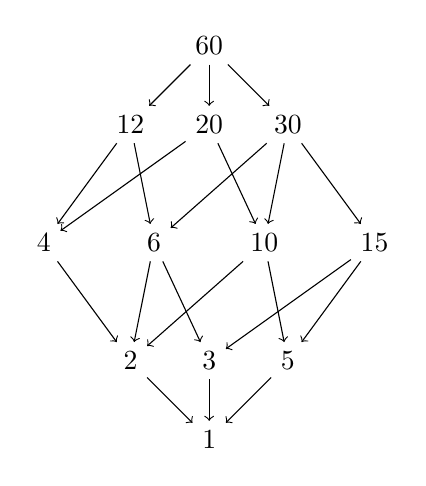
\begin{tikzpicture}
        \node (1) at (0,0) {1};

        \node (2) at (-1,1) {2};
        \node (3) at (0,1) {3};
        \node (5) at (1,1) {5};

        \node (4) at (-2.1,2.5) {4};
        \node (6) at (-0.7,2.5) {6};
        \node (10) at (0.7,2.5) {10};
        \node (15) at (2.1,2.5) {15};

        \node (12) at (-1, 4) {12};
        \node (20) at (0, 4) {20};
        \node (30) at (1, 4) {30};

        \node (60) at (0, 5) {60};

        \draw[->] (2) -- (1);
        \draw[->] (3) -- (1);
        \draw[->] (5) -- (1);

        \draw[->] (4) -- (2);
        \draw[->] (6) -- (2);
        \draw[->] (6) -- (3);
        \draw[->] (10) -- (2);
        \draw[->] (10) -- (5);
        \draw[->] (15) -- (3);
        \draw[->] (15) -- (5);

        \draw[->] (12) -- (4);
        \draw[->] (12) -- (6);
        \draw[->] (20) -- (4);
        \draw[->] (20) -- (10);
        \draw[->] (30) -- (6);
        \draw[->] (30) -- (10);
        \draw[->] (30) -- (15);

        \draw[->] (60) -- (12);
        \draw[->] (60) -- (20);
        \draw[->] (60) -- (30);
    \end{tikzpicture}
\end{center}

\de{
    Eine partielle Ordnung heißt \red{total} oder \red{linear}, falls je zwei Elemente vergleichbar sind, d.h. $\forall a,b \in A: a \le b \lor b \le a$
}

\ex \begin{itemize}
    \item $\le$ auf $\N, \Z, \Q, \R$
    \item $|$ auf $\{1,2,4,8,16,32,64,128,\dots\}$
    \item nicht $|$ auf $\N$
    \item nicht $\subseteq$ auf $P(A)$, falls $|A| \ge 2$
\end{itemize}

\lem{
    Sei A eine endliche Menge und R eine partielle Ordnung auf A.\\
    Dann gibt es eine totale Ordnung L auf A mit $R \subseteq L$.
}

\newpage
\pr{
    Falls R total ist, muss L auch total sein und wir sind fertig.

    Sonst seien $x,y \in A$ und unvergleichbar.\\
    Sei $R' := R \cup \{(u,v) \st (u,x), (y,v) \in R\}$. Dann ist $(x,y) \in R'$
    \begin{enumerate}
        \item R' ist reflexiv, da R reflexiv ist und eine Ordnung reflexiv bleibt, wenn zu ihr weitere Elemente hinzugefügt werden.
        \item R' ist antisymmetrisch: Sei $(a,b), (b,a) \in R'$.
        \begin{itemize}
            \item Falls $(a,b), (b,a) \in R$, dann ist a = b.
            \item Falls $(a,b) \in R$ und $(b,a) \notin R$, dann ist $(b,x),(y,a) \in R$, dann ist $(a,x), (y,b) \in R$, dann ist $(y,x) \in R$, was ein Widerspruch ist, also kann dieser Fall nicht existieren.
            \item Falls $(a,b),(b,a) \in R' \bs R$, dann ist $a = b$.
        \end{itemize}
        \item R' ist transitiv: Seien $(a,b),(b,c) \in R'$.
        \begin{itemize}
            \item Falls $(a,b),(b,c) \in R$, dann ist $(a,c) \in R$.
            \item Falls $(a,b),(b,c) \notin R$, dann ist $(a,x),(y,b),(b,x),(y,c) \in R$, dann ist $(x,y) \in R$, weshalb der Fall nicht existieren kann.
            \item Falls $(a,b) \in R$ und $(b,c) \notin R$, dann ist $(b,x),(y,c) \in R$, dann ist $(a,x),(y,c) \in R$.
        \end{itemize}
        Das heißt, das $R' \supseteq R$, also ist R' eine lineare Erweiterung von R.
    \end{enumerate}
}

\de{
    Sei A eine Menge. Eine Relation auf A heißt \red{Quasiordnung}, falls sie reflexiv und transitiv ist. Wir schreiben $a \preceq b$
}

Aus einer Quasiordnung bekommt man eine Äquivalenzrelation:
\[
    \sim := \{(a,b) \in A \times A \st a \preceq b \land b \preceq a\} = \preceq \cap \succeq
\]

\an{
    Falls $\preceq$ partiell ist, dann ist $\sim$ Gleichheit.
}

\de{
    Sei $\preceq$ eine Quasiordnung auf der Menge A und $\sim := \preceq \cap \succeq$. Dann ist die \red{Faktorordnung} von $\preceq$ die Ordnung auf $A / \sim$ definiert durch:
    \[
        a/\sim \le b/\sim \iff a \preceq b
    \]
}

\lem{
    $\le$ ist wohldefiniert und eine partielle Ordnung auf $A / \sim$.
}
\pr{
    \begin{itemize}
        \item wohldefiniert: Seien $a' \in a / \sim$ und $b' \in b / \sim$ und $a \preceq b$. Zu zeigen ist, dass gilt: $a' \preceq b'$.\\
        $a' \in a / \sim \implies a' \preceq a$ und $b' \in b / \sim \implies b' \preceq b$.\\
        $a' \preceq a \land b' \preceq b \implies a' \preceq b'$, denn $a' \preceq a \preceq b \preceq b'$.
        \item reflexiv: $a \preceq a \implies a / \sim \le a / \sim$
        \item anit-symmetrisch: Seien $b / \sim \in A / \sim$ mit $a / \sim \le b / \sim$ und $b / \sim \le a / \sim$.\\
        Dann ist $a \preceq b$ und $b \preceq a$, das heißt $a \sim b$ und $a / \sim = b / \sim$
    \end{itemize}
}

\ex Sei A die Menge der komplexen Zahlen und $z \preceq z' \iff |z| \le |z'|$. Es gilt: $z \sim z' \iff |z| = |z'|$.\\
$\exists$ Bijektion: $\R_{\ge 0} \to \C / \sim: x \mapsto x / \sim$.\\
Faktorordnung auf f: $\C / \sim \triangleq \le \text{ auf } \R$\\
Dies lässt sich grafisch als Kreise um den Urpsrung darstellen, wobei dies die Äquivalenzklassen sind.

\subsection{Ketten und Antiketten}

Sei $(A; \le)$ eine Menge mit partieller Ordnung.

\de{
    Eine Teilemenge $K \subseteq A$ heißt
    \begin{itemize}
        \item \red{Kette}, falls $\forall a,b \in K: a \le b \lor b \le a$
        \item \red{Antikette}, falls $\forall a,b \in K: a \le b \implies a = b$
    \end{itemize}
}

\de{
    Eine \red{aufsteigende Kette}, ist eine Abbildung $f: I \in \N \to A$ mit $i \le j \implies f(i) \le f(j)$.\\
    Eine \red{absteigende Kette}, ist eine Abbildung $f: I \in \N \to A$ mit $i \le j \implies f(i) \ge f(j)$.
}

\se{
    Sei A eine unendliche Menge und $\le$ eine partielle Ordnung auf A.\\
    Dann gibt es auf A eine unendliche Kette oder eine unendliche Antikette.
}

\ex $(\N; \st)$
\begin{itemize}
    \item unendlich aufsteigende Kette: $(1,2,4,8,16,\dots)$, $f: \N \to \N: f(i) = 2^i$
    \item unendliche Antikette: $(2,3,5,7,11,13,\dots)$, alle Primzahlen
    \item es gibt keine unendlich absteigende Kette
\end{itemize}

\subsection{Ordnungen auf Wörtern}

\de{
    Sei A eine endliche Menge, z.B. $A = \{a,b,\dots,z\}$.\\
    Ein \red{Wort der Länge n} ist eine Abbildung $W: \{1, \dots, n\} \to A$.\\
    z.B.: $W(1,2,3,4) = h,u,n,d$
    \begin{itemize}
        \item $|W| := n$ ist die Länge des Wortes W
        \item $\epsilon = 0$ ist ein Wort der Länge 0
        \item $A*$ ist die Menge aller Wörter über A
    \end{itemize}
}

\de{
    Wir definierten drei Ordnungen auf A:
    \begin{itemize}
        \item Präfixordnungen
        \item Teilwortordnungen
        \item Lexikographische Ordnungen
    \end{itemize}
}

\subsubsection{Präfixordnungen}

\de{
    Seien $U,V \in A*$. Dann ist U ein \red{Präfix von V}, falls
    \begin{itemize}
        \item $|U| \le |V|$
        \item $\forall i \le |U|: U(i) = V(i)$
    \end{itemize}
    Zum Beispiel ist "mathe" ein Präfix von "mathematik".\\
    Das zugehörige Hasse-Diagramm ist ein unendlicher Baum.
}

Es gibt
\begin{itemize}
    \item unendlich aufsteigende Ketten: (a, aa, aaa, \dots)
    \item keine unendlich absteigenden Ketten
    \item unendliche Antiketten, falls $|A| \ge 2$: (a, ba, bba, bbba, \dots)
\end{itemize}

\subsubsection{Lexikographische Ordnungen}

\de{
    Sei $\le$ eine totale Ordnung auf A, z.B. $a \le b \le c \le \dots \le z$. Seien $U,V \in A*$.\\
    Dann ist U \red{lexikographisch kleiner als} V, falls
    \begin{itemize}
        \item U ein Präfix von V ist oder
        \item sei i die kleinste Zahl mit $U(i) \ne V(i)$, dann $U \le V \iff U(i) \le V(i)$
    \end{itemize}
}

\subsubsection{Teilwortordnungen}

\de{
    Seien $U, V \in A*$. Dann ist U ein Teilwort von V, wenn man U durch Wegstreichen von Buchstaben aus V erhält,\\
    d.h. $\exists 1 \leq i_1 \leq i_2 \leq \dots \leq i_{|U|} \leq |V|: U(j) = V(j)$ für $1 \leq j \leq |U|$\\
    z.B. mathematik $\to$ \sout{m}at\sout{h}em\sout{atik} $\to$ atem
}

\an{
    Falls U ein Teilwort von V ist, gilt: $U \leq V$
}

\an{
    Es gibt keine Antiketten
}

\newpage
\section{Bäume zählen}

\se{
    Für $n \geq 1$ gibt es $n^{n-2}$ Bäume mit Knotenmenge $\{1, \dots, n\}$.
}

\subsection{Prüfercodes}

\de{
    Sei $B = (V,E)$ ein endlicher Baum mit $V \subseteq E$. Der \red{Prüfercode} von B lässt sich eindeutig induktiv berechnen:
    \begin{itemize}
        \item $|V| = 2: P(B) = \emptyset$
        \item $|V| \ge 2:$ Sei b das kleinste Blatt von B, $a_1$ der Nachbar von B und $w := P((V \bs \{b\}), (E \bs \{a_1, b\}))$. Dann gilt $P(B) = a_1w$
    \end{itemize}
}

\an{
    Der Prüfercode ist ein Wort der Länge $|V| - 2$ im Alphabet V. Die Buchstaben die nicht vorkommen, sind genau die Blätter von B.
}

\ex
\begin{itemize}
    \item $B = (V,E)$ mit $V = \{1,2,3,4,5\}$ und $E = \{\{1,2\}, \{2,3\}, \{3,4\}, \{3,5\}\}$\\
    Prüfercode: 234
    \item $B = (V,E)$ mit $V = \{1,2,3,4,5,6\}$ und\\
    $E =  \{\{1,2\}, \{1,3\}, \{1,4\}, \{1,5\}, \{1,6\}\}$\\
    Prüfercode: 1111
\end{itemize}

Umgekehrt erhalten wir aus einem Prüfercode einen Baum:\\
Sei $w = a_1, \dots, a_{n-2}$ ein Wort in $\{1, \dots, n\}$
\begin{itemize}
    \item Falls $w =\emptyset: B = (\{1,2\}, \{\{1,2\}\})$
    \item Sonst: Konstruiere ein Wort $b_1, \dots, b_{n-2}$ mit
    \begin{itemize}
        \item Sei $b_1$ das kleinste Element von $V \bs \{a_1, \dots, a_{n-2}\}$.
        \item Für $i \in \{1, \dots, n-3\}$ sei $b_{i+1}$ das kleinste Element aus\\
        $V \bs \{b_1, \dots, b_i, a_{i+1}, \dots, a_{n-2}\}$.
        \item Sei $e = V \bs \{b_1, \dots, b_{n-2}\}$.
    \end{itemize}
    Dann ist $E = \{\{a_1, b_1\}, \dots, \{a_{n-2}, b_{n-2}\}, e\}$ und $V = \{1, \dots, n\}$.
\end{itemize}

\newpage
\se{
    Jedes Wort der Länge $n-2$ in den Buchstaben $\{1, \dots, n\}$ ist\\
    Prüfercode genau eines Baumes mit Kantenlänge $V := \{1, \dots, n\}$
}
\pr{
    Induktion über n:\\
    \underline{$A_n$} ist die Aussage: Sei $|V| = n$. Dann ist jedes Wort in V der Länge $n-2$ ein Prüfercode genau eines Baumes mit Knotenmenge V.

    \underline{$n = 2$:} Klar, da es nur einen Baum mit zwei Knoten gibt.\\
    \underline{$n \geq 3$:} Nach IV ist $a_1, \dots, a_{n-3}$ der Prüfercoe eines Baumes B' mit Knotenmenge $V \bs \{b_1\}$, wobei $b_1$ das kleinste Element von\\
    $V \bs \{a_1, \dots, a_{n-3}\}$ ist.\\
    Die Blätter von B' sind $(V \bs \{b_1\}) \bs \{a_1, \dots, a_{n-3}\}$, d.h. $b_1$ ist kleiner als alle Blätter von B' $\iff B := (V, (B') \cup \{\{a_1, b_1\}\})$ hat den Prüfercode $a_1P(B')$.
}

\subsection{Spannbäume}

\de{
    Sei $G = (V,E)$ ein Graph. Ein \red{Spannbaum} von G ist ein Subgraph B von G mit
    \begin{itemize}
        \item $V(B) = V$
        \item B ist ein Baum
    \end{itemize}
}

Jeder endliche zusammenhängende Graph hat einen Spannbaum. Um diesen zu erhalten werden solange Kanten aus Kreisen gelöscht, bis keine Kreise mehr vorhanden sind.

\de{
    Sei $G = (V,E)$ ein endlicher Graph.\\
    \red{$\tau(G)$} bezeichnet die Anzahl der Spannbäume von G.
}

\ex \begin{itemize}
    \item $\tau(G) = 0 \iff G$ ist nicht zusammenhängend
    \item $\tau(G) = 1 \iff G$ ist ein Baum
    \item $\tau(C_n) = n$
    \item $\tau(K_n) = n^{n-2}$
\end{itemize}

\subsection{Adjazenzmatrix}
\de{
    Sei $G = (\{1, \dots, n\}, E)$ ein Graph. Die \red{Adjazenzmatrix} von G ist die Matrix $A = (a_{ij})_{i,j \in \{1, \dots, n\}}$ mit $a_{ij} = \begin{cases}
        1 & \text{falls } \{i,j\} \in E\\
        0 & \text{sonst}
    \end{cases}$

    Die \red{Gradmatrix} von G ist die Diagonalmatrix $D = (d_{ij})_{i,j \in \{1, \dots, n\}}$ mit $d_{ii} = \deg(i)$
}

\an{
    \begin{itemize}
        \item A und D sind symmetrisch: $A^T = A$ und $D^T = D$.
        \item Spalten- und Zeilensummen von A sind der Grad:
        \[
            d_{ii} = \sum_{i=i}^{n} a_{ij} = \sum_{j=1}^{n} a_{ij} = \deg(i)
        \]
    \end{itemize}
}

\se{
    Sei $n \geq 2$ und $G = (\{1, \dots, n\}, E)$ ein Graph, A die Adjazenzmatrix von G und D die Gradmatrix von G. Sei $i \in \{1, \dots, n\}$.\\
    Dann gilt: $\tau(G) = \det(D-A)_{ii}$.
}

\de{
    Sei A eine $n \times 1$-Matrix und $i \in \{i, \dots, n\}$.\\
    Dann ist $A_i$ die Matrix, die entsteht, wenn die i-te Zeile und Spalte von A entfernt werden.
}

\ex $D-A = \begin{pmatrix}
    2 & -1 & -1 & 0\\
    -1 & 2 & -1 & 0\\
    -1 & 1 & -3& 1\\
    0 & 0 & -1 & 1
\end{pmatrix}$.

$\det(D-A)_{33} = \det(\begin{pmatrix}
    2 & -1 & 0\\
    -1 & 2 & 0\\
    0 & -1 & 1
\end{pmatrix}) = \det(\begin{pmatrix}
    2 & -1\\
    -1 & 2
\end{pmatrix}) = 4 - 1 = 3$

\subsubsection{Multigraphen}

\de{
    Ein \red{Multigraph} ist ein Tripel $(V, E, i)$ mit $V \cap E = \emptyset$\\
    mit $i : E \to \{\{a,b\} \st a,b \in V\}$.\\
    \gray{
        Somit können Schleifen und Kantendopplungen auftreten.
    }
}

\ex $V = \{1\}, E = \{a,b\}, i: E \to \vvec{V}{2} \cup \vvec{V}{1}$

\end{document}
